\documentclass[12pt,a4,english,finnish,pdflatex%,handout
]{beamer}
\definecolor{MyGreen}{RGB}{50, 120, 50}
\usecolortheme[named=MyGreen]{structure}
\usefonttheme{serif}

\usepackage{babel}
\usepackage[utf8]{inputenc}
\usepackage[T1]{fontenc}
\usepackage{amsmath,amssymb} 
\usepackage{animate}
\usepackage{multimedia}

\usepackage{natbib}
\bibpunct[: ]{(}{)}{,}{}{}{;}

\usepackage{tikz}

\usepackage{tipa}

\usepackage{hyperref}

\usepackage{graphicx}

\setbeamertemplate{navigation symbols}{}

\graphicspath{{figures/}}

\setlength{\leftmargini}{0pt}
\setlength{\leftmarginii}{1em}

\newcommand{\kommentti}[1]{
  {\bf[#1]}
}

\author{Pertti Palo} 

\begin{document}
\title{Analysing Articulatory Data with Vector Norms and Related Methods}
\date{9 Oct 2023} 

\frame{\titlepage
  \centering
} 

\frame{\frametitle{Outline}
  \begin{itemize}
    \item Introduction
    \item Ultrasound tongue imaging
    \item Pixel Difference (PD)
    \item PD and other methods applied
	\begin{itemize}
	    \item PD on de-interlaced lip videos
	    \item Metrics on tongue splines
	    \item PD on 3D/4D ultrasound
	    \item PD on Raw vs Interpolated 2D data
	    \item Choosing the norm or metric for PD
	\end{itemize}
    \item MRI
  \end{itemize}
}


\frame{\frametitle{Introduction}
  \begin{itemize}
  \item Pre-speech articulation is interesting from several points of view, but
  analysing ultrasound videos manually is not great.
  \item In my thesis I concentrated on timing of utterance onset in both
  acoustics and articulation \citep{Palo-MeasuringPrespeechArticulation-2019}.
  \item The data was high-speed tongue ultrasound from a delayed naming
  experiment -- specifically one using the Rastle instructions
  \citep{RastleEtAl-CharacterizingMotorExecution-2005}.
  \end{itemize} 

 	\centering
	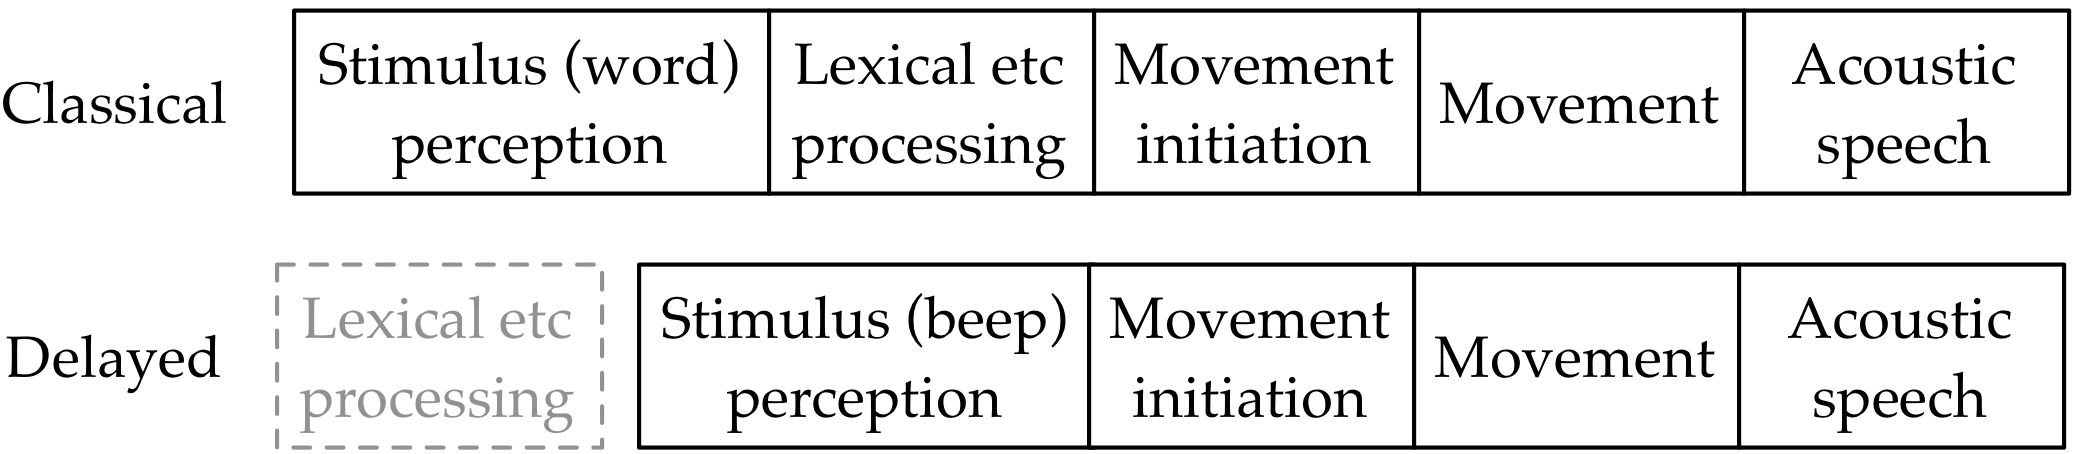
\includegraphics[width=\textwidth]{figures/stages_of_naming.jpg}
}


\frame{\frametitle{Introduction}
  \begin{itemize}
  \item When trying to identify movement onset in greyscale videos with a lot of
  speckle 'noise', it doesn't take long to grow a desire for an easier way.
  \item The speckle 'noise' maybe caused by a number of factors including bubbles in the 
  acoustic gel between the chin and the probe, and more interestingly changes in internal 
  structures of tissues -- such as muscle fibres tensing and relaxing.
  \end{itemize} 
  
  
}

\frame{\frametitle{Ultrasound tongue imaging: What is imaged?}
	\centering
	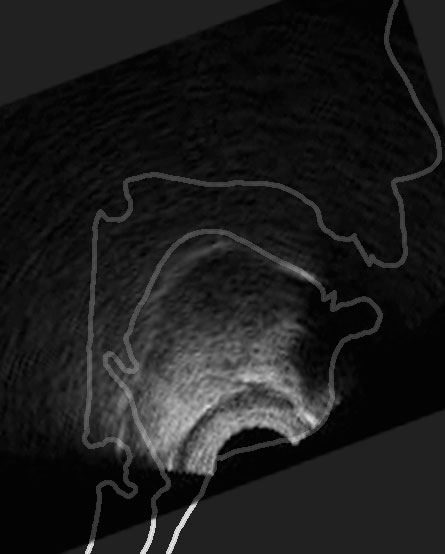
\includegraphics[width=0.45\linewidth]{figures/DA_and_P1_overlay_2}
	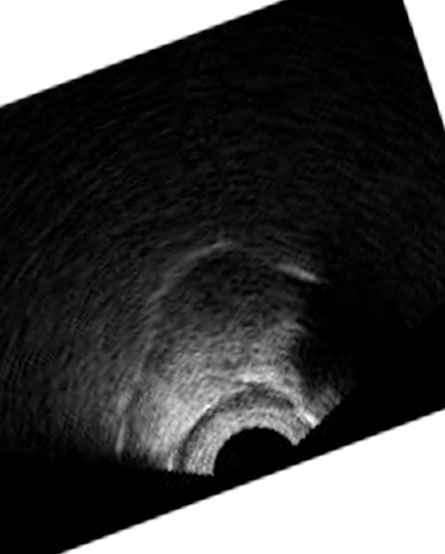
\includegraphics[width=0.45\linewidth]{figures/DA_and_P1_overlay_3}
}

\frame{\frametitle{Ultrasound tongue imaging: Extracting a spline}

	\centering
	\hspace*{-.75cm}
	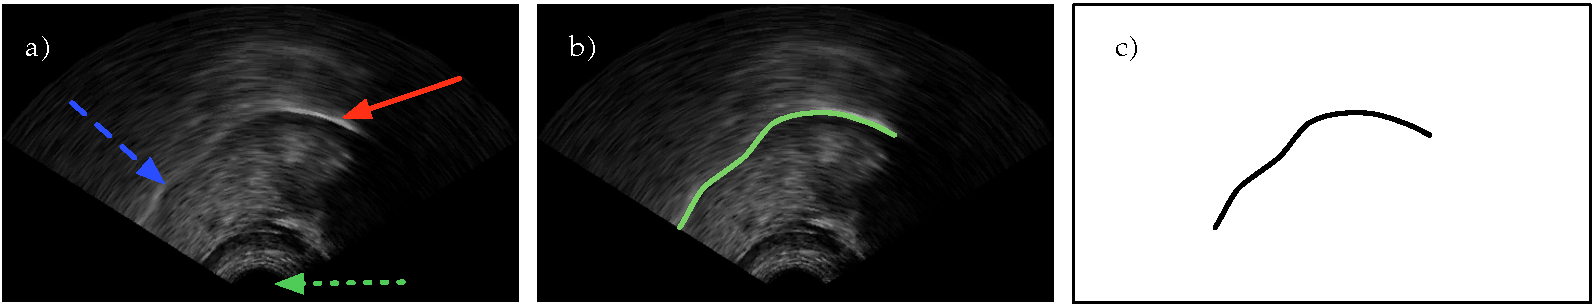
\includegraphics[width=1.125\linewidth]{P2_lemon_1st_frame_spline.pdf}
}

\frame{\frametitle{Ultrasound tongue imaging: parameters}

\begin{itemize}
	\item 2D ultrasound has good time resolution: 80-120 fps in today's examples.
	\item Usually, 2D ultrasound is used in the mid-sagittal plane.
	\item 3D/4D ultrasound can image the tongue as a volumetric object, but at
	the cost of lower frame rates: typically about 20 fps.
	\item Both have fairly good -- but slightly complex -- spatial resolution.
\end{itemize}
}

\frame{
  \centering
  {
    \bf \Large 
    \usebeamercolor[fg]{title}
    The main method
    
    \vfill
%    \includegraphics[height=1.5cm]{figures/aalto_logo} 
  }
}



\frame{\frametitle{Pixel Difference (PD)}
	\begin{itemize}
	\item The first tool out of the box happened to work adequately --  and so for my
	thesis I used Euclidean distance or $l2$-norm to identify articulatory onsets.
	\end{itemize}


	\centering
	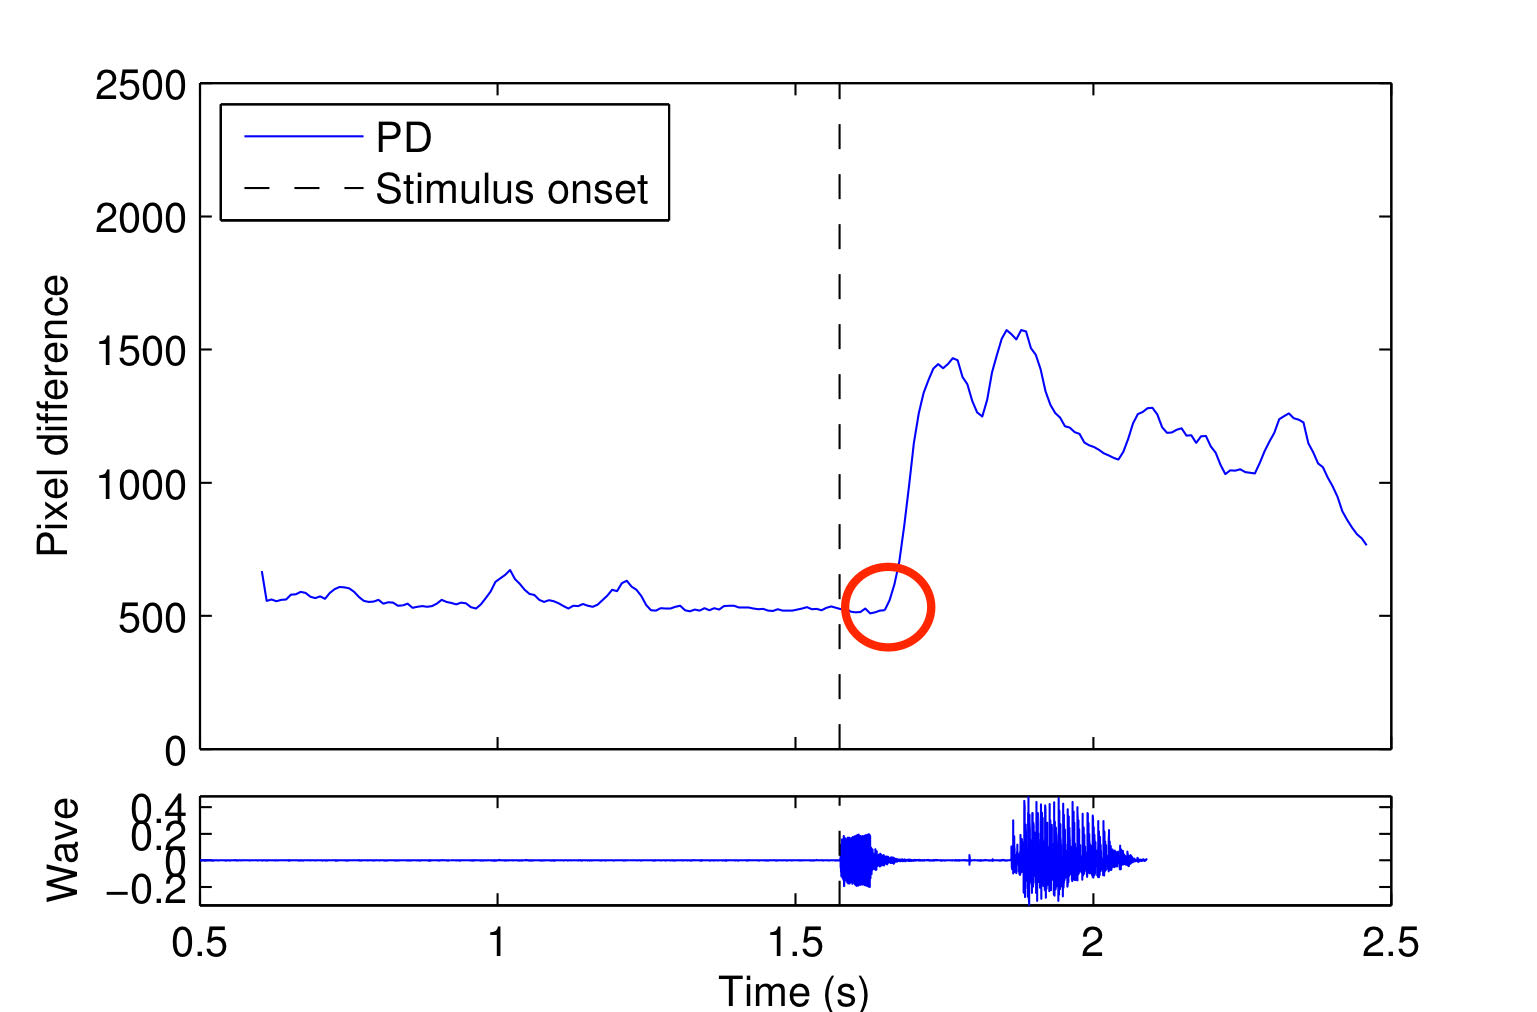
\includegraphics[height=.7\textheight]{figures/pd_caught.jpg}
}

\frame{\frametitle{Pixel Difference (PD): Background}
	\begin{itemize}
		\item The analysis methods presented here are similar to methods
		developed by
		\begin{itemize}
			\item
			 \cite{McMillanCorley-CascadingInfluencesProduction-2010} and
			 \cite{DrakeEtAl-ARTICULATORYEVIDENCEINVOLVEMENT-2013} who used
			 Euclidean distance on ultrasound frames and
			\item \cite{RaeesyEtAl-ParametrisingDegreeArticulator-2011} who
			 used a similar method on MRI data.
		\end{itemize}
		\item The way I have used it, it is actually just the Pythagorean
			theorem applied in a space with a lot more dimensions than 2.
		\end{itemize}
}

\frame{\frametitle{Pixel Difference (PD): Raw vs. Interpolated}
	\begin{itemize}
		\item PD is usually calculated on 
		\begin{itemize}
			\item (a) uninterpolated (probe-return) ultrasound data instead of
			\item (b) interpolated (human-readable) data.
		\end{itemize}
	\end{itemize}
	\centering
	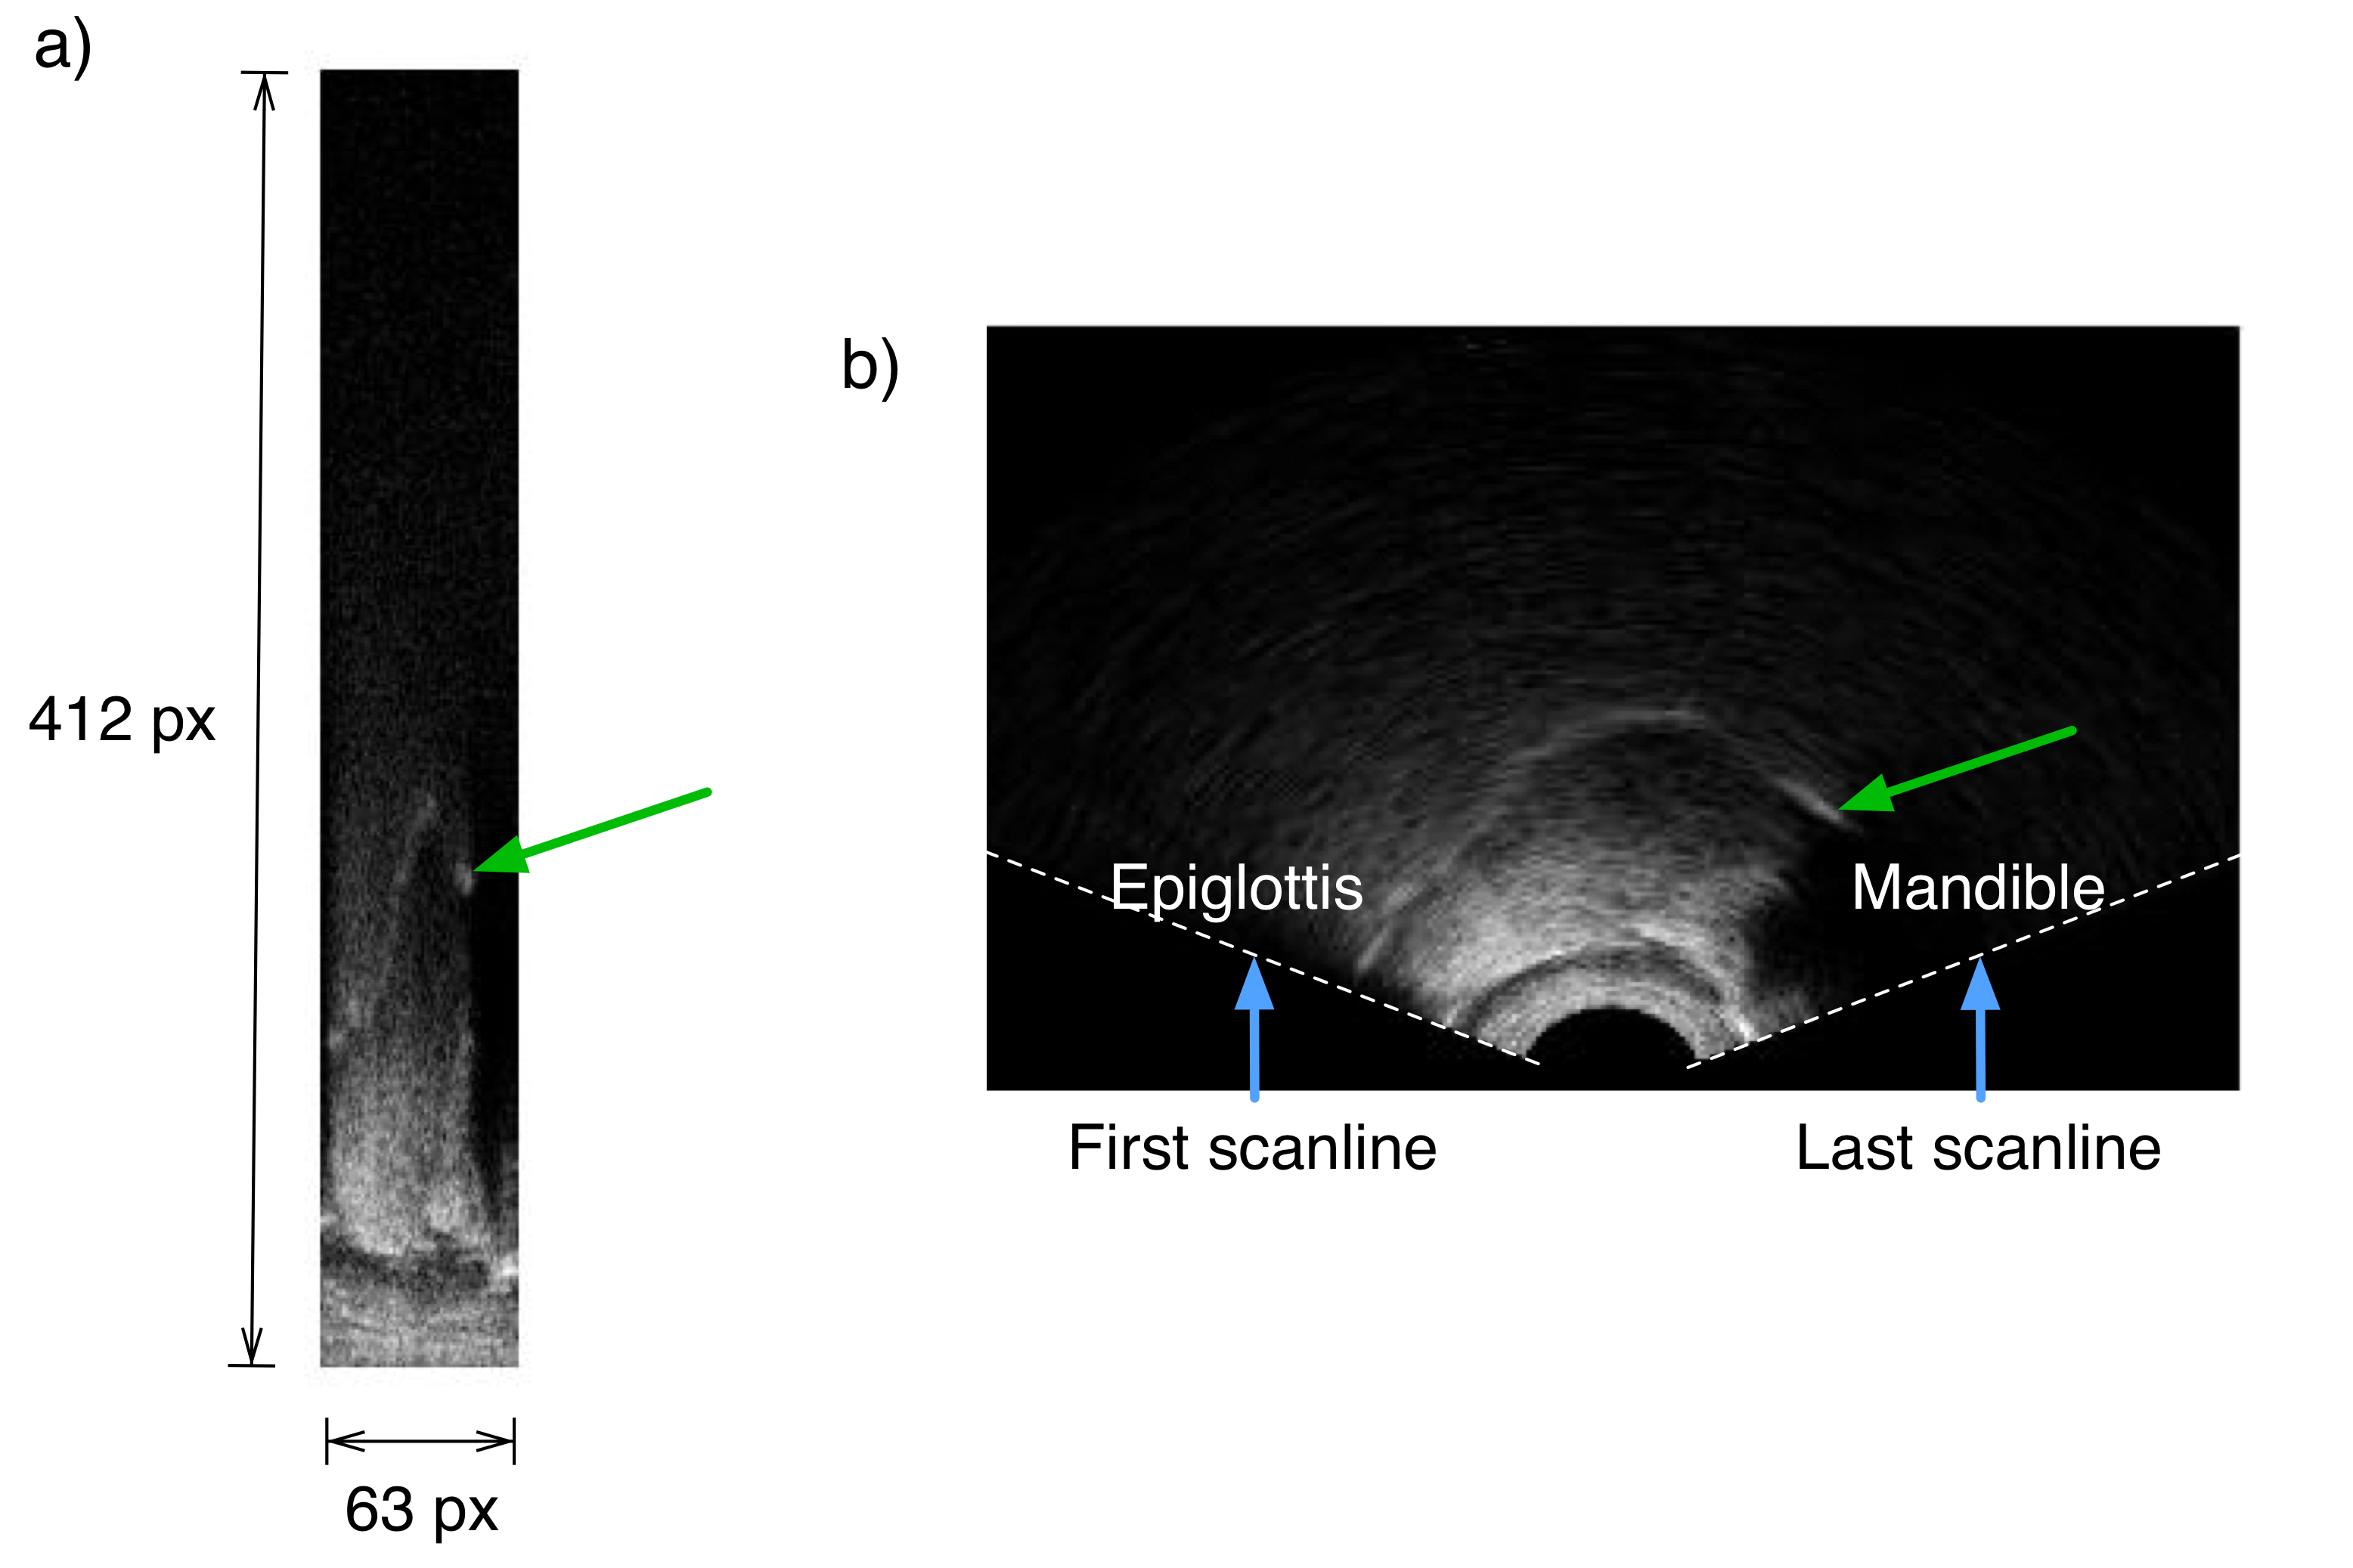
\includegraphics[height=.7\textheight]{figures/raw_and_interpolated.jpg}

	}

\frame{\frametitle{Pixel Difference (PD): The maths}
	\begin{equation*}
	l2(t+0.5) = \sqrt{\sum_{i, j} (x(i,j,t+1) - x(i,j,t))^2}
	\end{equation*}

	\begin{itemize}
		\item $i$ and $j$ are indices that span the width and height of the
		image, $t$ is the time index.
		\item Like said, this is actually just the Pythagorean theorem applied
		in a space with a lot more dimensions than 2.
	\end{itemize}

	}

\frame{\frametitle{Pixel Difference (PD): The maths visually}
	\centering
	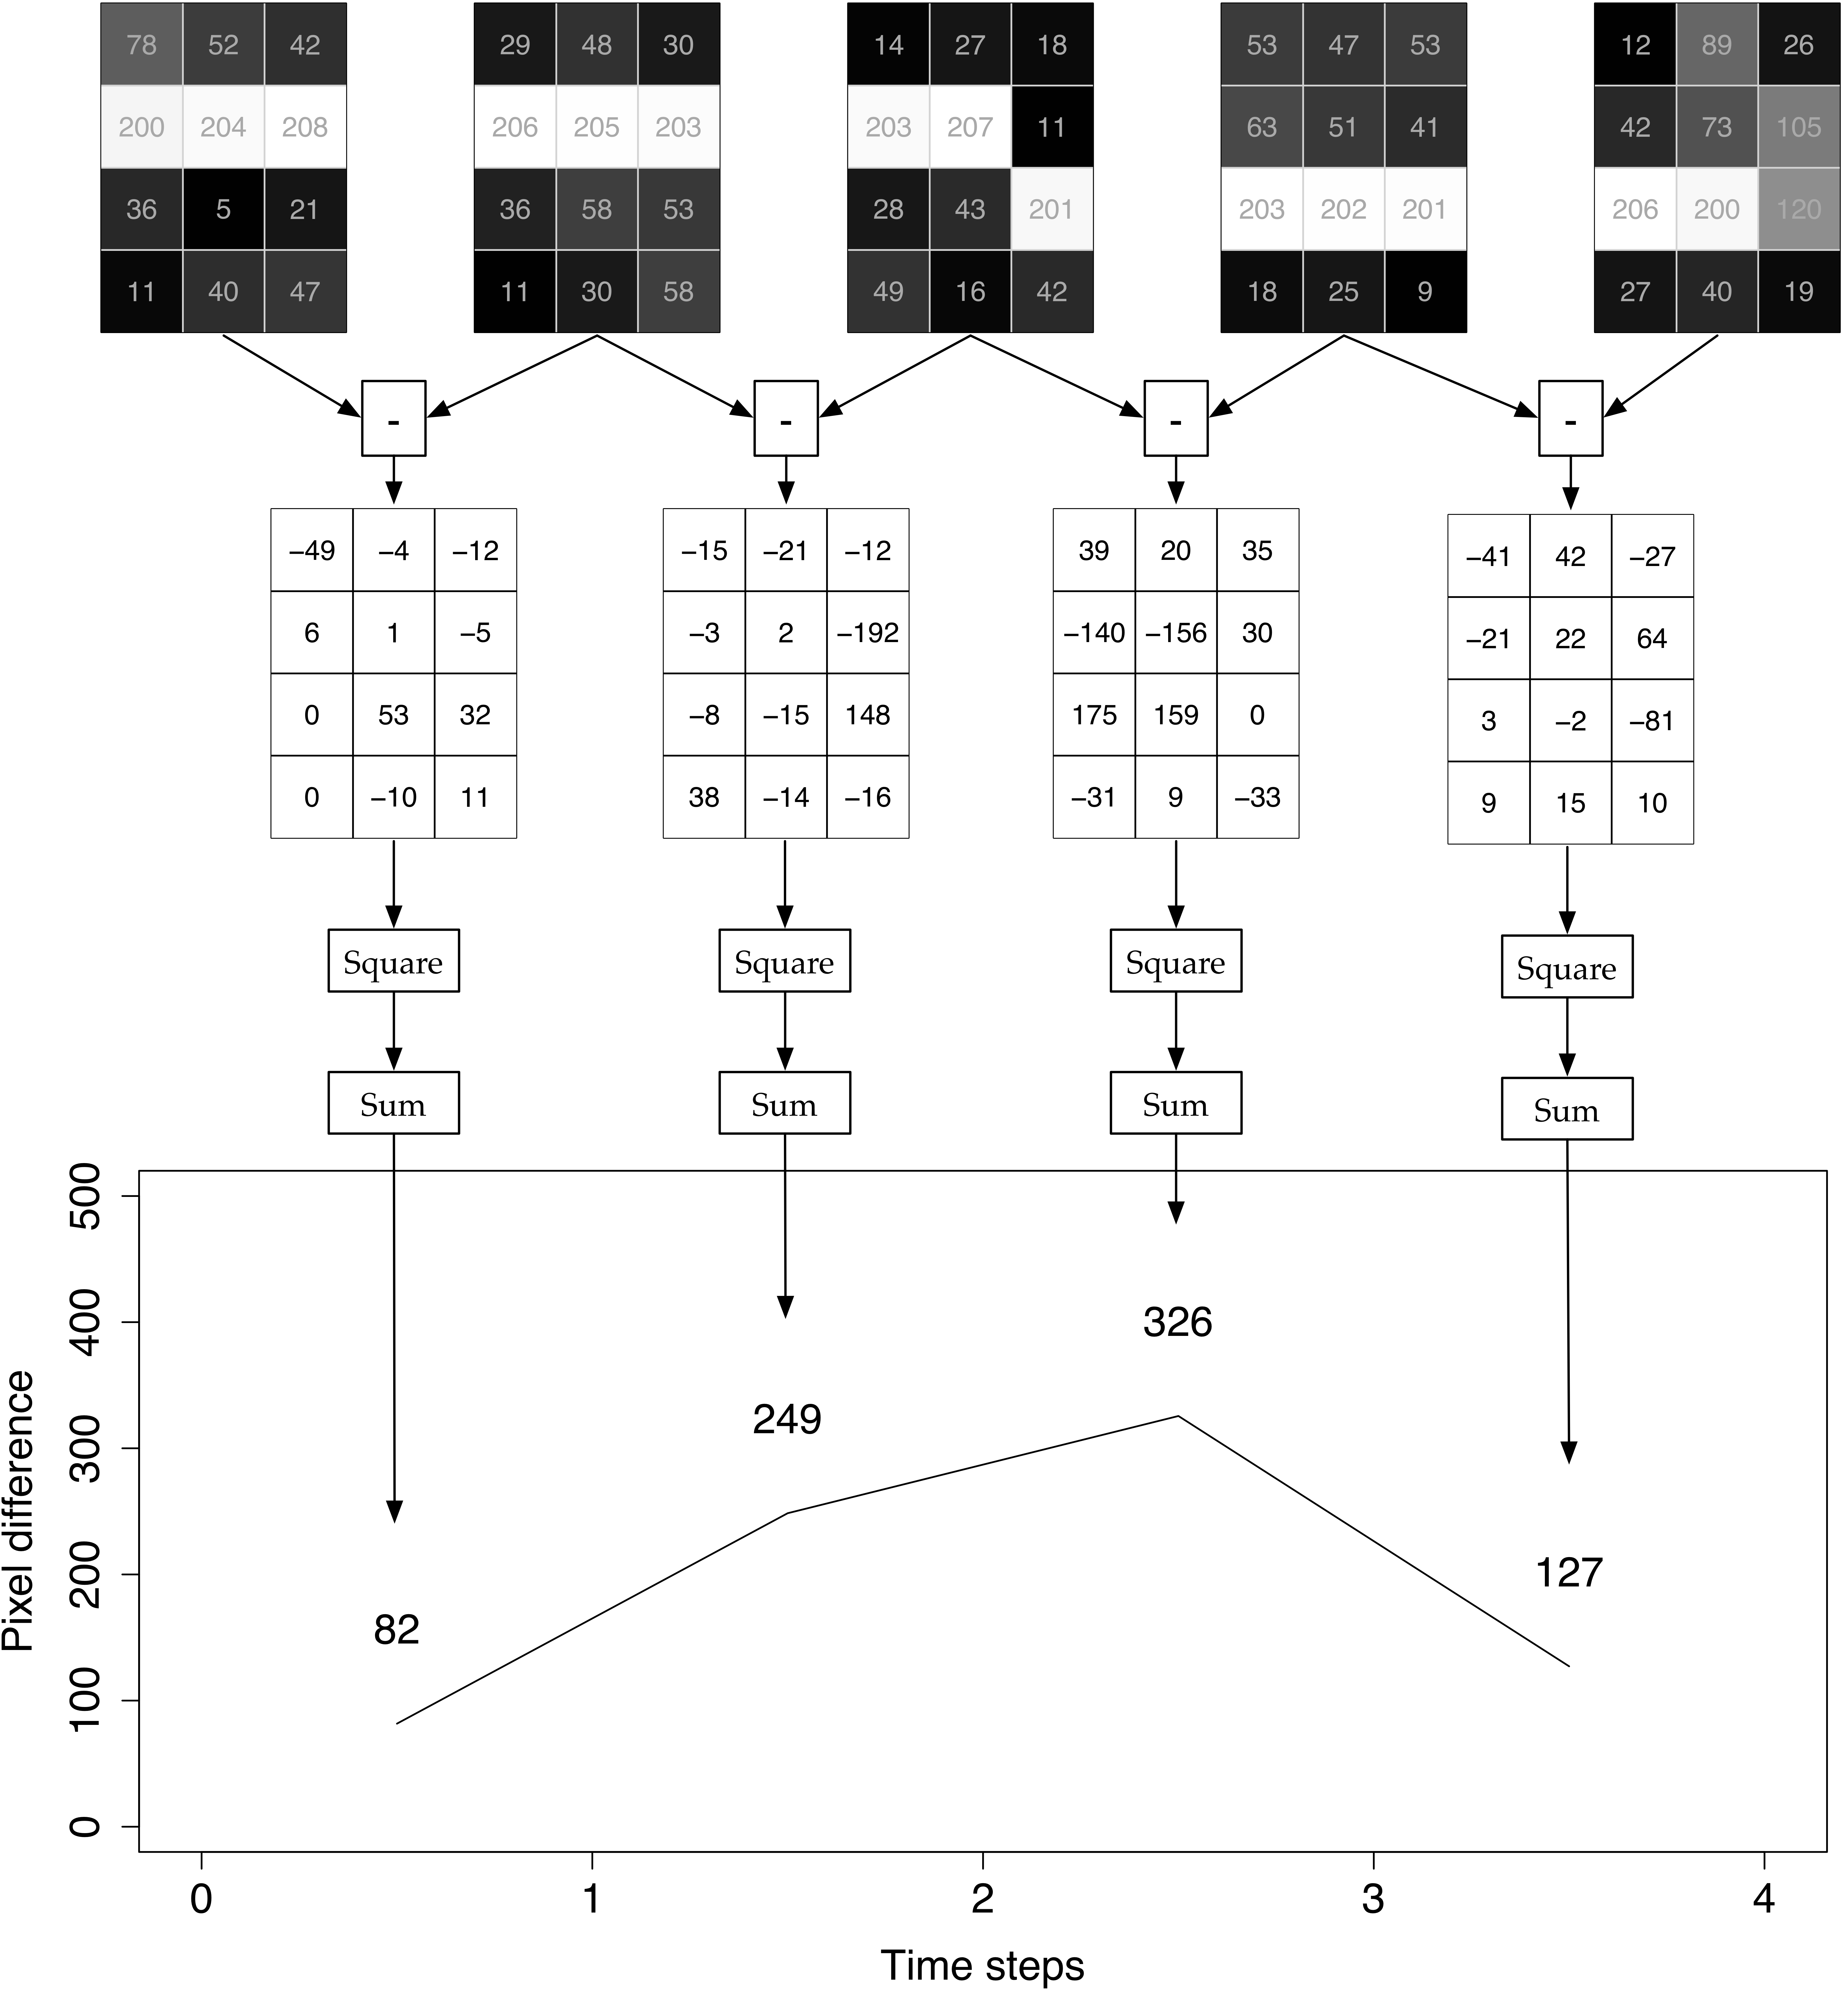
\includegraphics[height=.8\textheight]{figures/pixel_difference_demo_noise_square_sum_tall.png}
}

\frame{
  \centering
  {
    \bf \Large 
    \usebeamercolor[fg]{title}
    PD and other metrics applied to articulatory data
    
    \vfill
%    \includegraphics[height=1.5cm]{figures/aalto_logo} 
  }
}

\frame{\frametitle{PD on de-interlaced videos}
	% A slowed down and up-close example of interlacing by Wikipedia user Grayshi.
	Lip video de-interlaced at 59.94 fps.
	\centering
	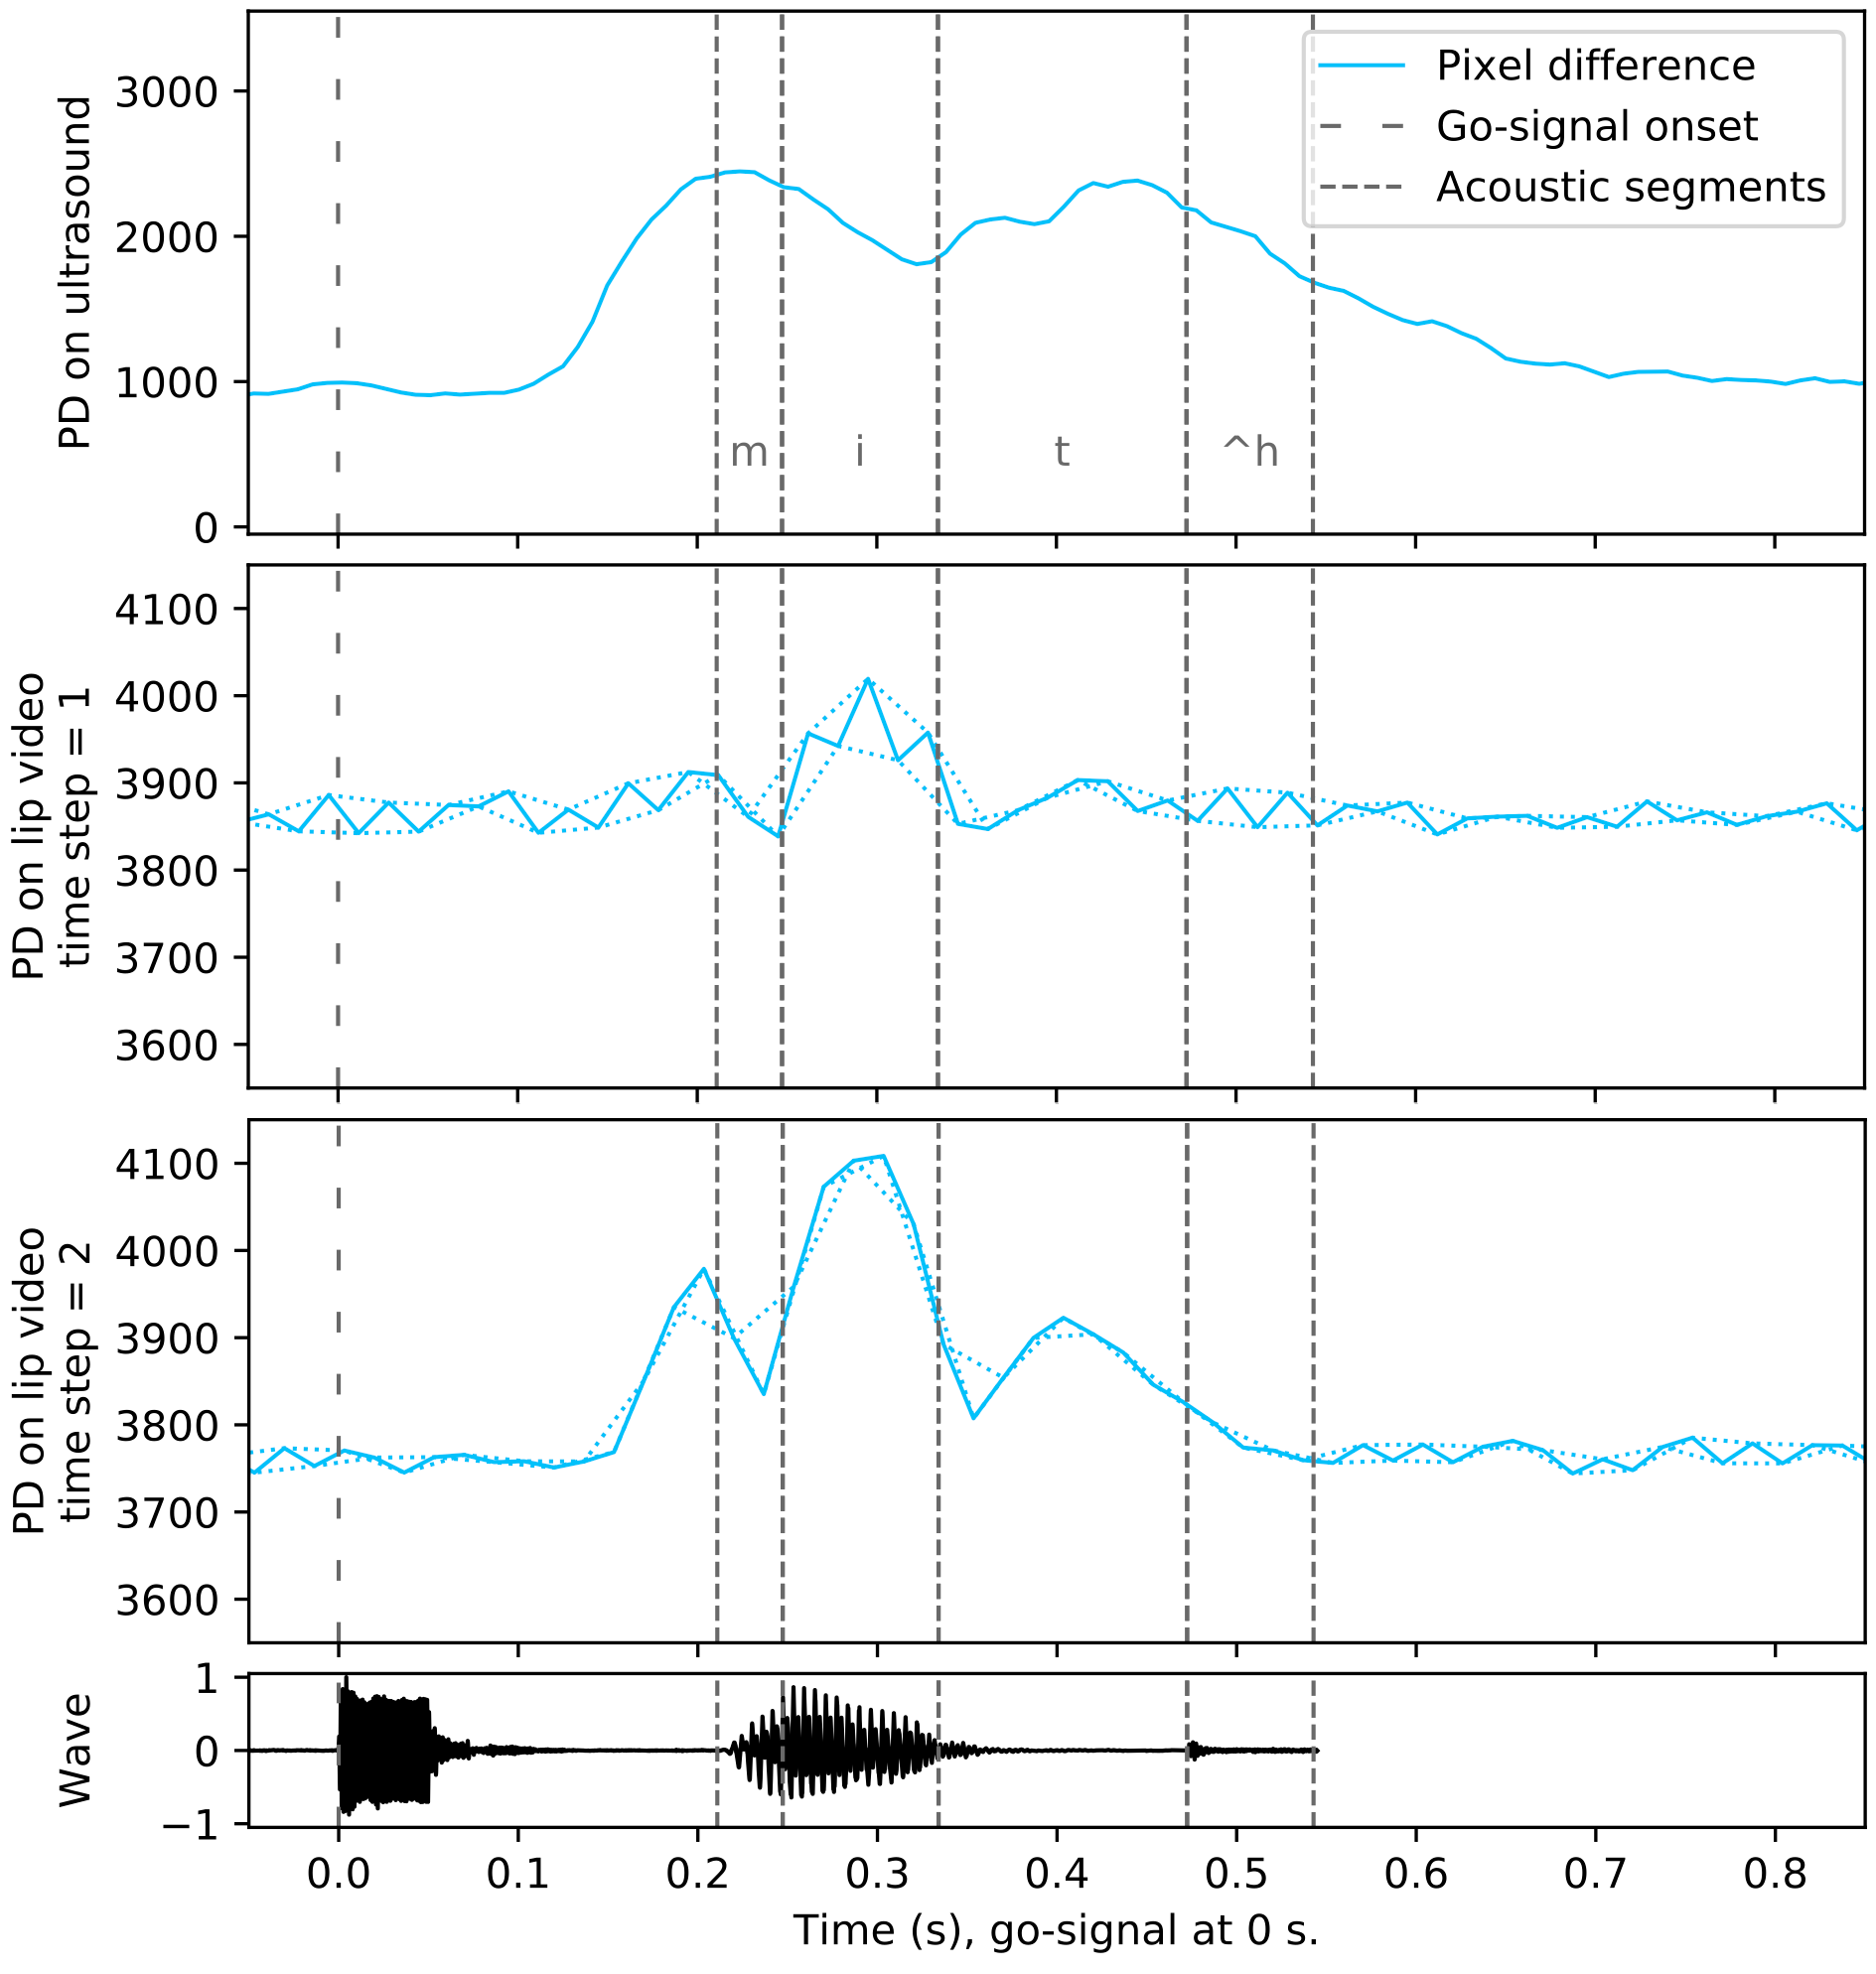
\includegraphics[width=0.7\linewidth]{figures/File127_pd_ult_and_vid_ts1_2.png}	
}

\frame{\frametitle{PD on de-interlaced videos}
	% A slowed down and up-close example of interlacing by Wikipedia user Grayshi.

	\begin{itemize}
		\item The graphic below demonstrates taking a time step of 1 vs 3 on
		ultrasound. 
		\item I tried that for my PhD thesis
		\citep{Palo-MeasuringPrespeechArticulation-2019}, but found that for
		ultrasound a time step of 1 is preferable.
		\item For de-interlaced videos the best time step is 2
		\citep{Palo-ComputerAssistedSegmentation-2021}.		
	\end{itemize}
	\vspace*{.5cm}
	\centering
	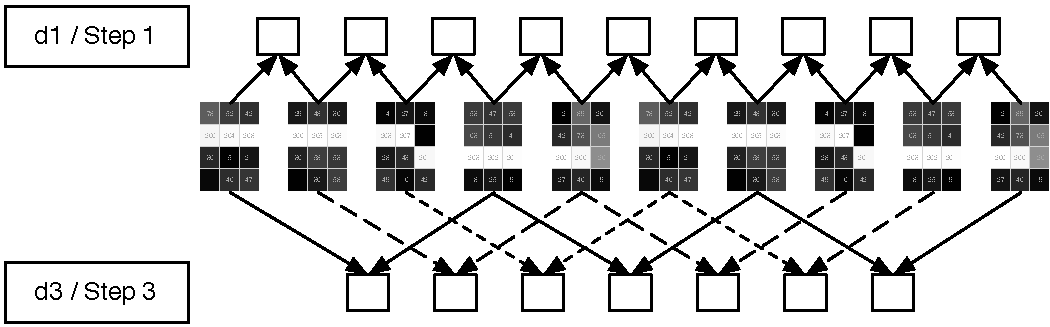
\includegraphics[width=\linewidth]{figures/d1_and_d3.pdf}

}

\frame{\frametitle{Tongue splines: Problems from spatial sparseness}

	\textbf{Raw ultrasound:} 
	\begin{itemize}
		\item Typically on the order of 10k pixels per frame, today 63x412
		pixels per frame.
		\item Individual pixel's fluctuations get averaged out.
	\end{itemize}

	\vspace{.25cm}
	\textbf{Tongue splines:}
	\begin{itemize}
		\item Typically on the order of 30-50 control points per frame, today
		42 control points per frame.
		\item Individual point's fluctuations may end up driving the data.
	\end{itemize}
	
	\vspace{.25cm}
	\centering
	\hspace*{-.75cm}
	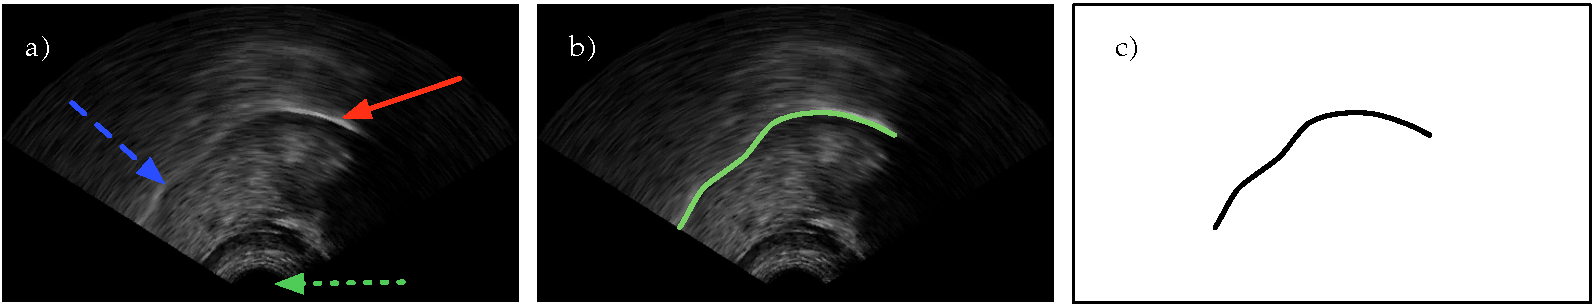
\includegraphics[width=1.125\linewidth]{P2_lemon_1st_frame_spline.pdf}

}

\frame{\frametitle{Tongue splines: Problems from spatial sparseness}

	\begin{itemize}
		\item Longer time step and averaging improve the results.
		\item Here and in the next slide ANND
		\citep{ZharkovaHewlett-MeasuringLingualCoarticulation-2009} and MPBPD
		\citep{Palo-CanWeDetect-2020} have been calculated with time step 3 and
		smoothed with a moving average filter with a 5 frame window.
	\end{itemize}

	\centering
	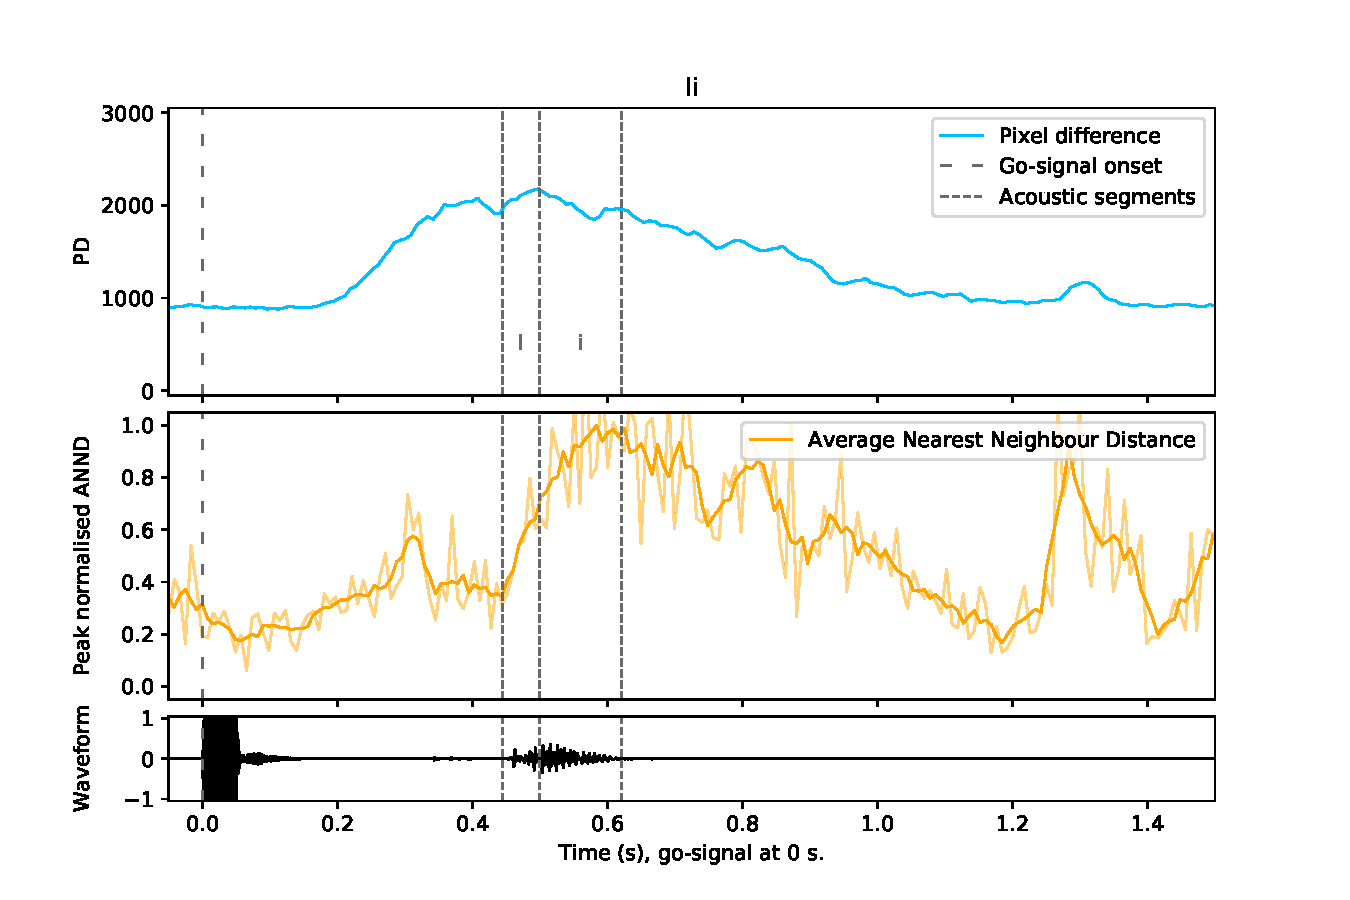
\includegraphics[width=.8\linewidth]{figures/File120_annd_pd}
}

\frame{\frametitle{Tongue splines: Problems from spatial sparseness}

	\begin{itemize}
	\item Choice of metric can help, but not with everything.
	\end{itemize}

	\centering
	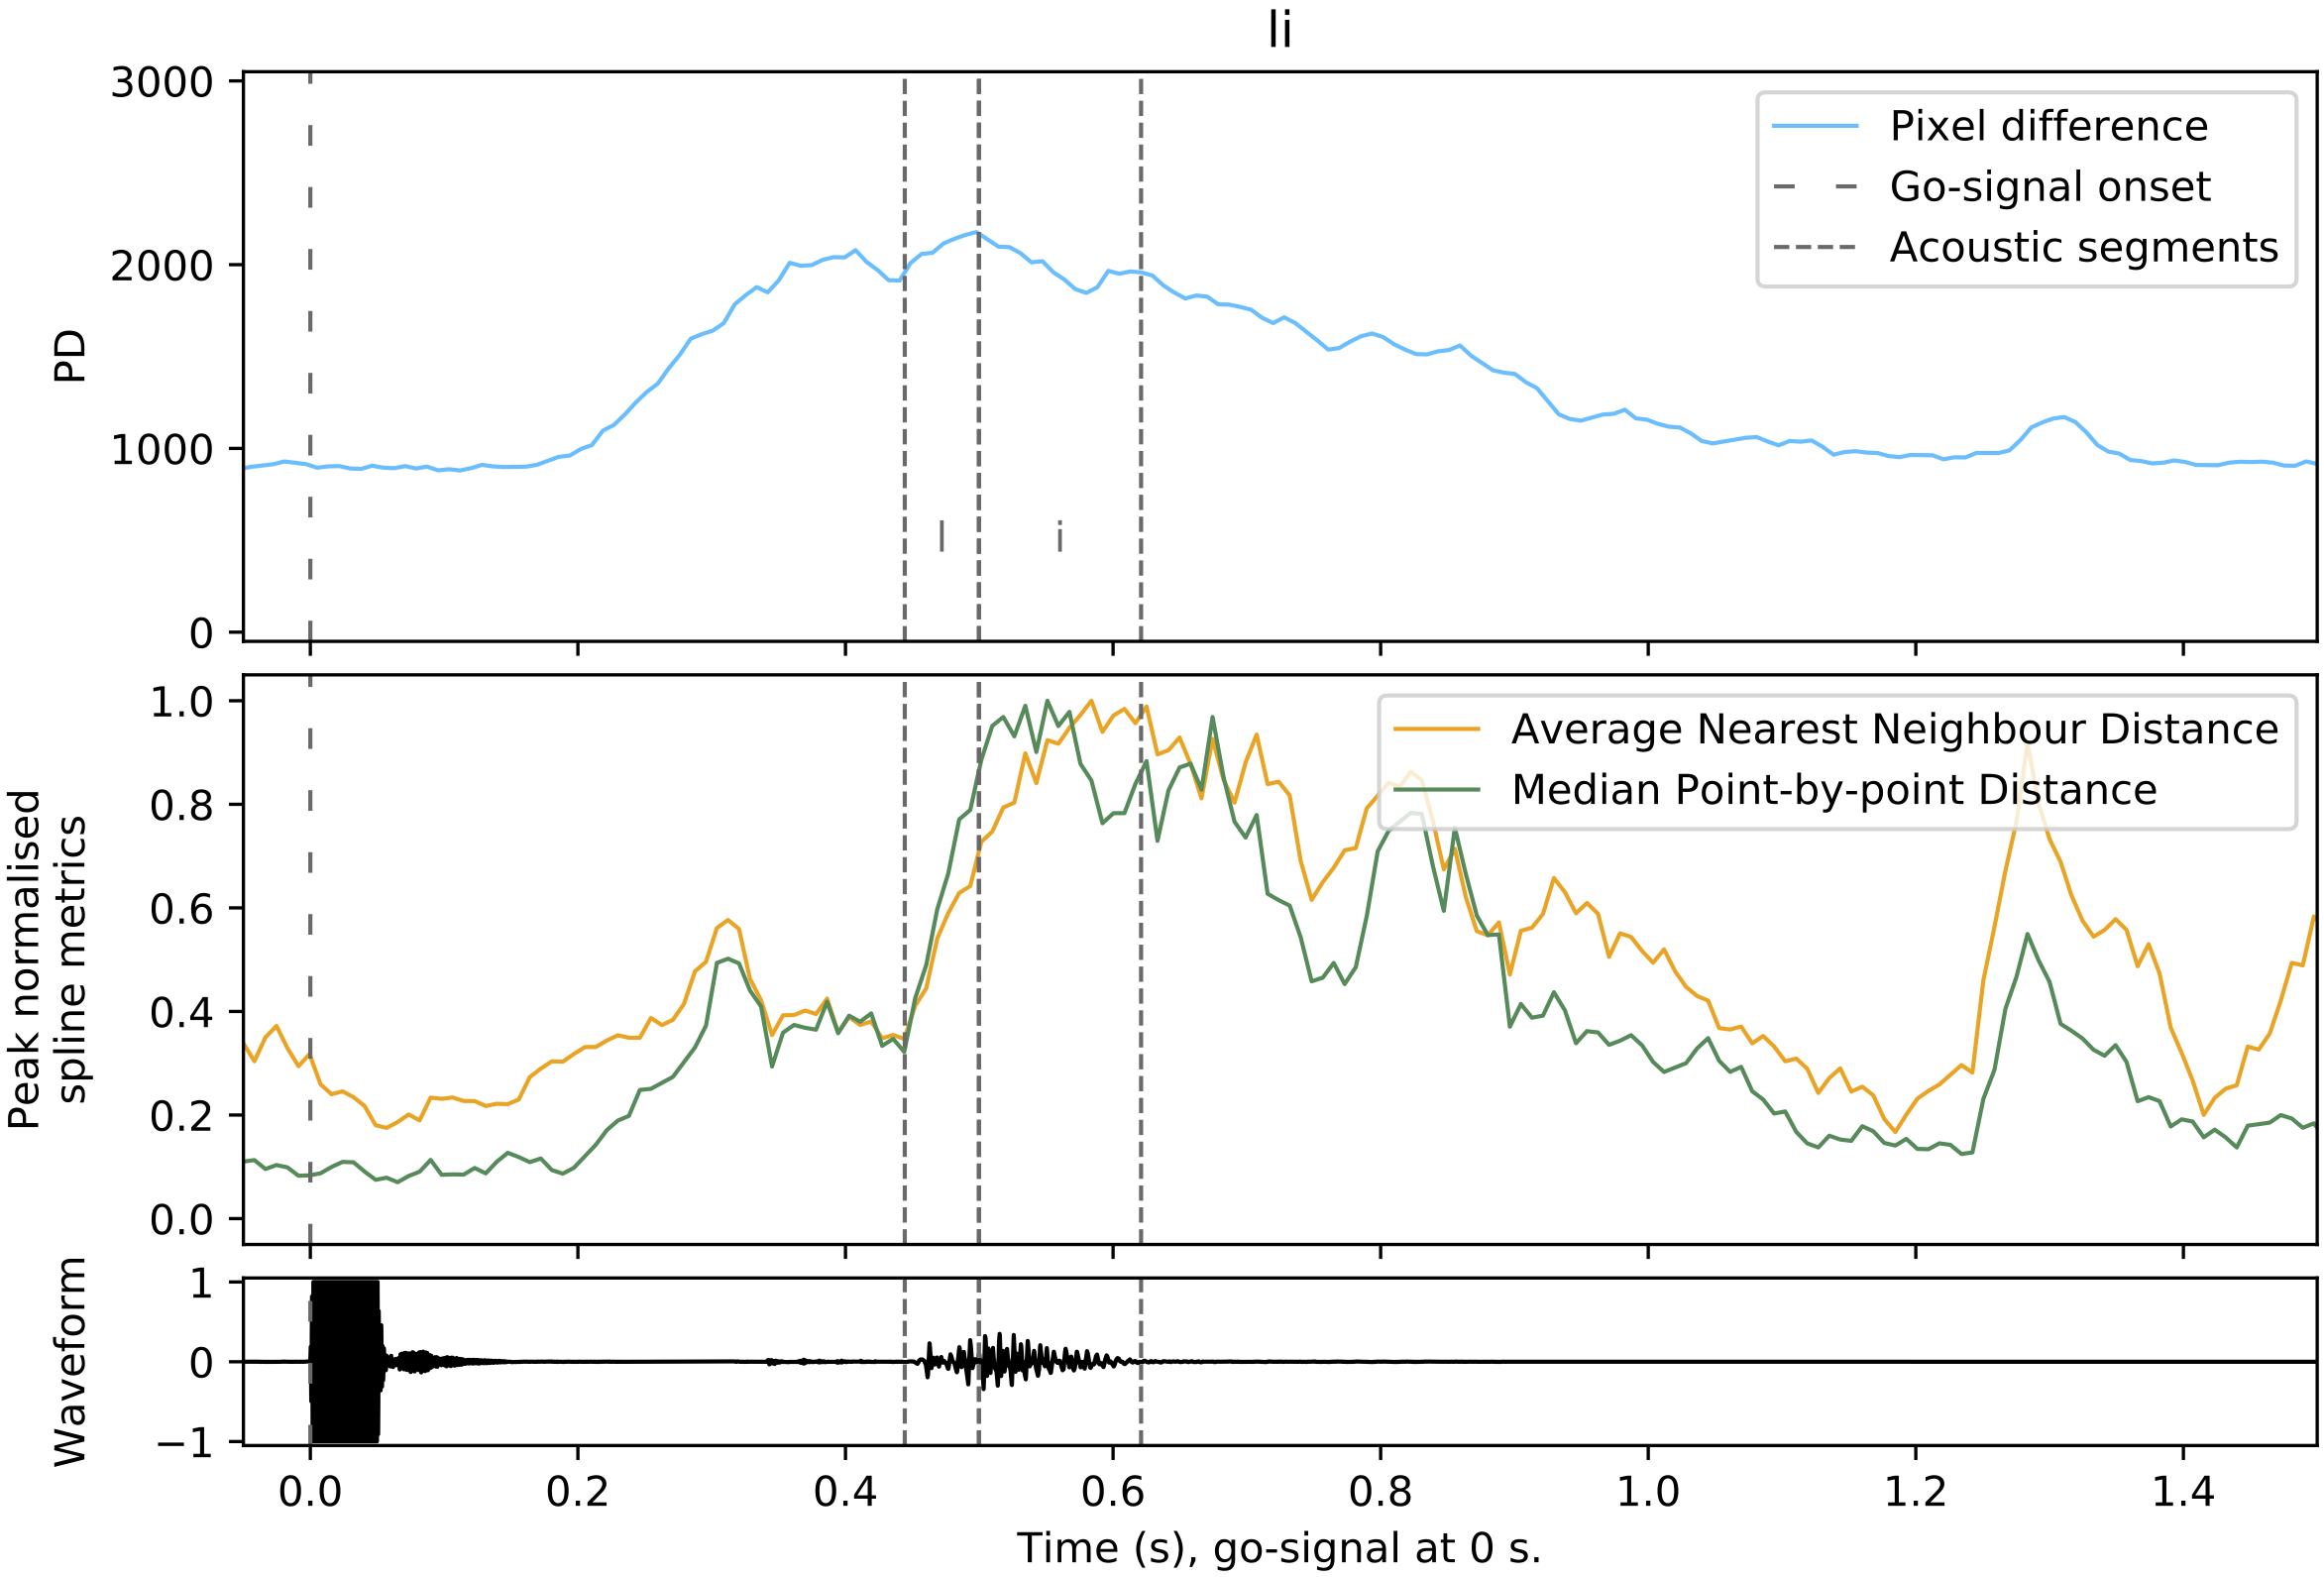
\includegraphics[width=\linewidth]{figures/File120_annd_mpbpd_pd}
	
}

\frame{\frametitle{3D/4D ultrasound}
	
	\begin{itemize}
		\item Capturing a 3D frame takes a lot longer.
		\item The images are always interpolated.
		\item In analysis even on good (lucky) samples onset and gesture recognition becomes difficult.
	\end{itemize}
	
	\begin{figure}
	\centering
	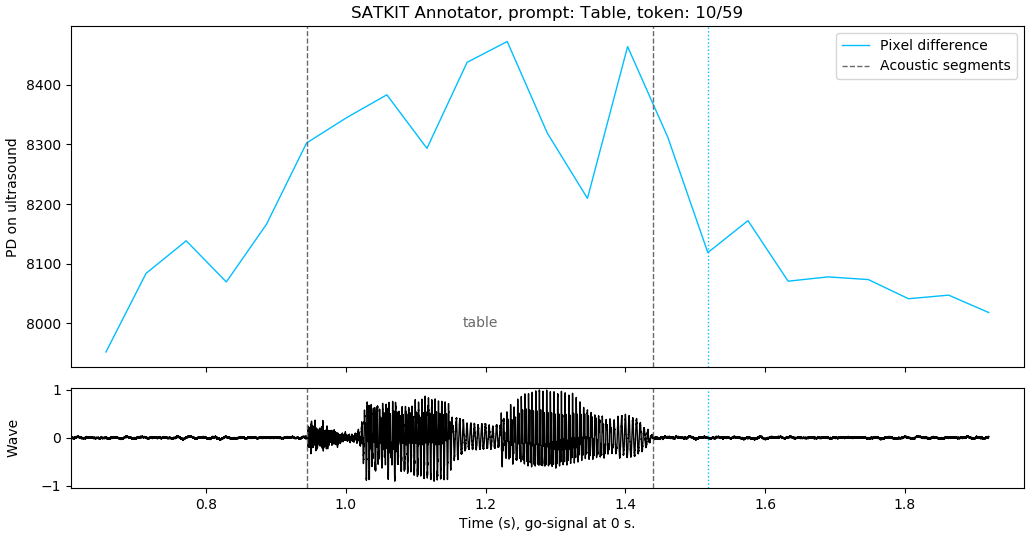
\includegraphics[width=.9\linewidth]{figures/PD_on_3D_cropped.png}	
	\end{figure}
	
}

\frame{\frametitle{PD on Raw vs Interpolated 2D data}
	
	\centering
	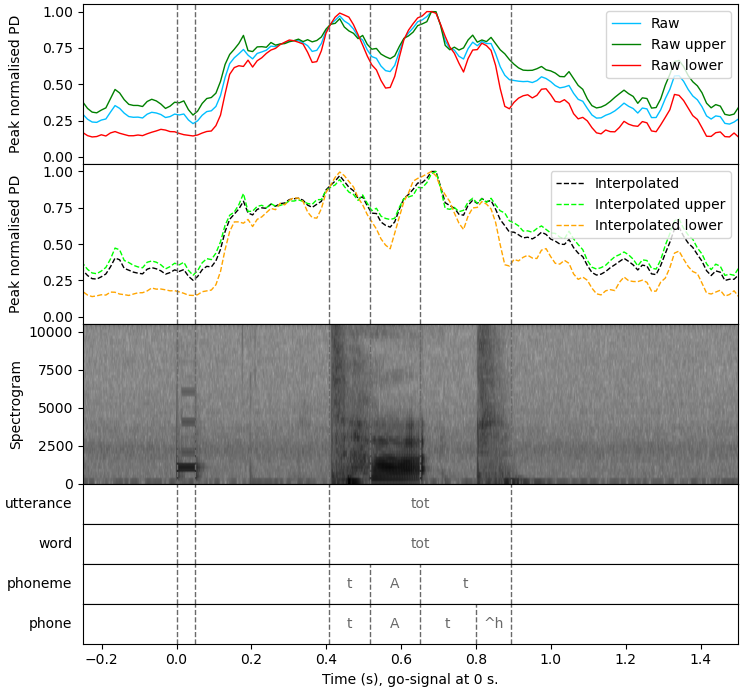
\includegraphics[width=.8\linewidth]{figures/raw_interpolated_2D}
}

\frame{\frametitle{PD on data with artificially lowered frame rate}
	\centering
	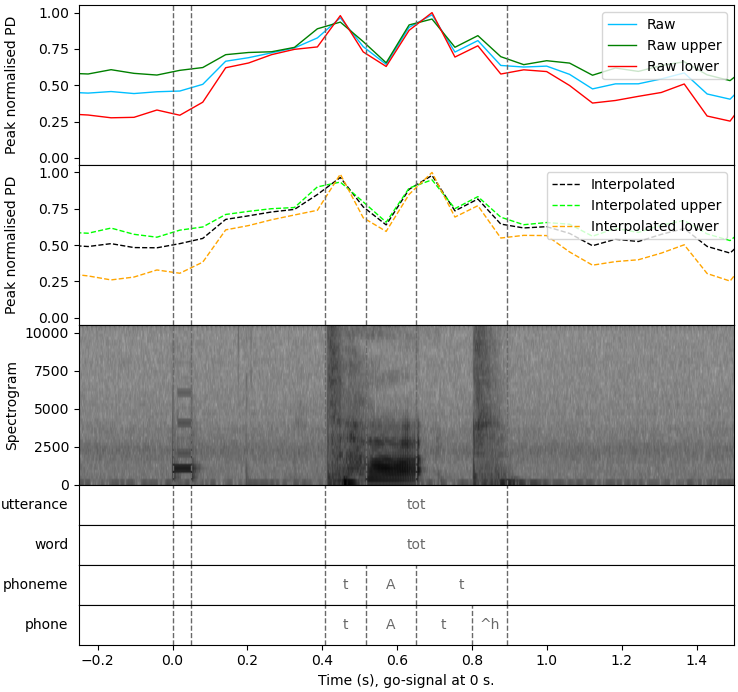
\includegraphics[width=.8\linewidth]{figures/raw_interpolated_2D_step5}
	
}

\frame{\frametitle{In the works: Choosing the metric for PD}
	\begin{itemize}
		\item PD has so far usually been calculated as the Euclidean distance or $l2$-norm.
		\item We've recently been looking at principled ways of selecting the norm for a given data source -- such as 2D ultrasound -- from the different $lp$-norms where $p \in \mathopen]0,\inf\mathclose[$. 
		\item It looks like the optimal norm for 2D ultrasound is $l1$ (or close to it):
	\end{itemize}	
	\begin{equation*}
		l1(t+0.5) = \sum_{i, j} |x(i,j,t+1) - x(i,j,t)|
	\end{equation*}
}

\frame{\frametitle{MRI: Challenges and how to deal with them}
	\begin{itemize}
		\item Frame rate can be a problem.
		\item If there are systematic changes frame-to-frame caused by the
		imaging and reconstruction these may show up in PD analysis.
		\item Best way to get ahead with using PD for analysis would be to get
		a small pilot sample and run the basic version on it: $l2$ or
		$l1$-norm, time step = 1, no smoothing.
		\item Apply larger time steps and smoothing if needed.
		\item Test different norms and/or look to different metrics all
		together.
	\end{itemize}
}

\frame{\frametitle{MRI: What makes it exciting?}
	
	\begin{itemize}
		\item Triangulation is always good: One view is no view.
		\item MRI can observe structures that are otherwise really difficult to
		image.
		\item Fast imaging sequences should be able to deal with the frame rate
		issues.
		\item Metrics like PD work well on data with fairly dense spatial
		resolution.  
	\end{itemize}
	
	
}

\frame{
  \centering
  {
    \bf \Large 
    \usebeamercolor[fg]{title}
    Thank you! Do you have questions?
    
    \vfill
%    \includegraphics[height=1.5cm]{figures/aalto_logo} 
  }
}


\frame{\frametitle{References}
  
\scriptsize
\bibliographystyle{apalike}
\bibliography{science_combined.bib}

}

\frame{
  \centering
  {
    \bf \Large 
    \usebeamercolor[fg]{title}
    Extra material
    
    \vfill
%    \includegraphics[height=1.5cm]{figures/aalto_logo} 
  }
}

\frame{\frametitle{Speech Articulation ToolKIT}
	
	\begin{itemize}
		\item \url{https://github.com/giuthas/satkit}.
		\item Written in Python and in active development.
	\end{itemize}
	
	\begin{figure}
		\centering
		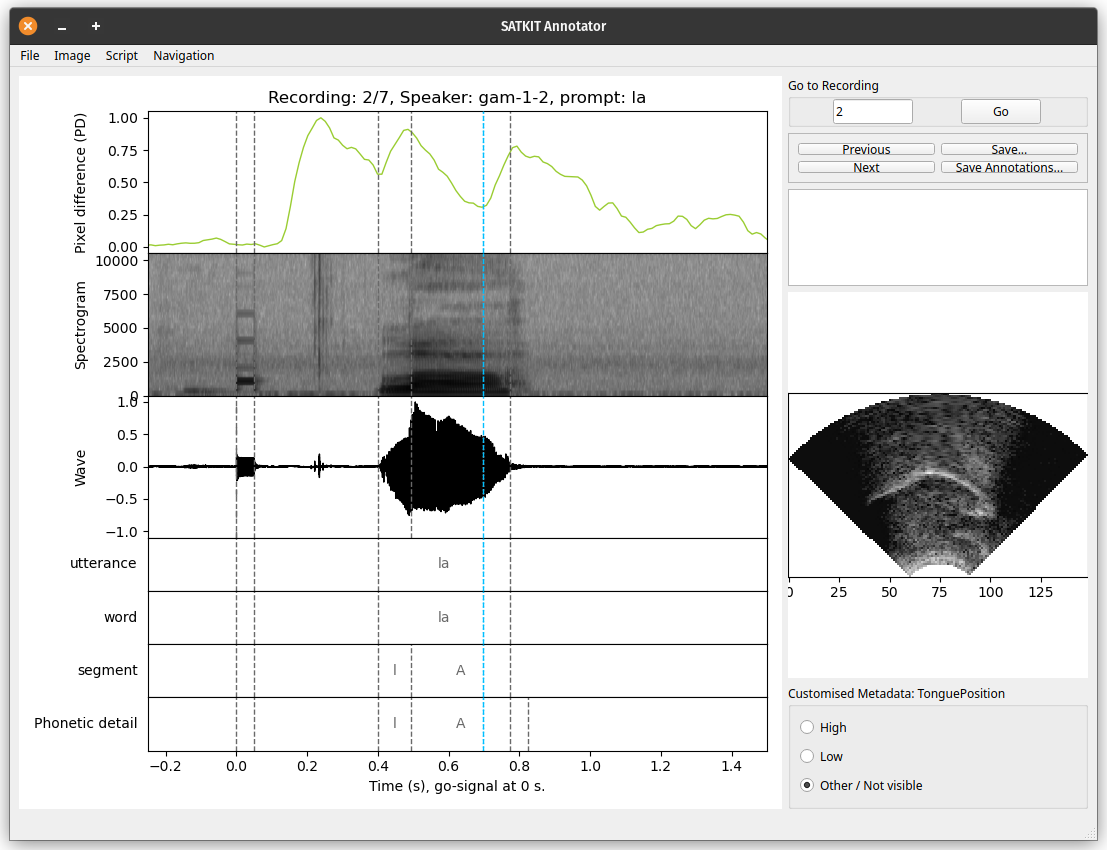
\includegraphics[width=.85\linewidth]{figures/SATKIT_UI.png}	
	\end{figure}	
}

\frame{\frametitle{Delayed naming results: Acoustics}
	\begin{center}
		\vspace*{-.5cm}
		\hspace*{-1cm}
		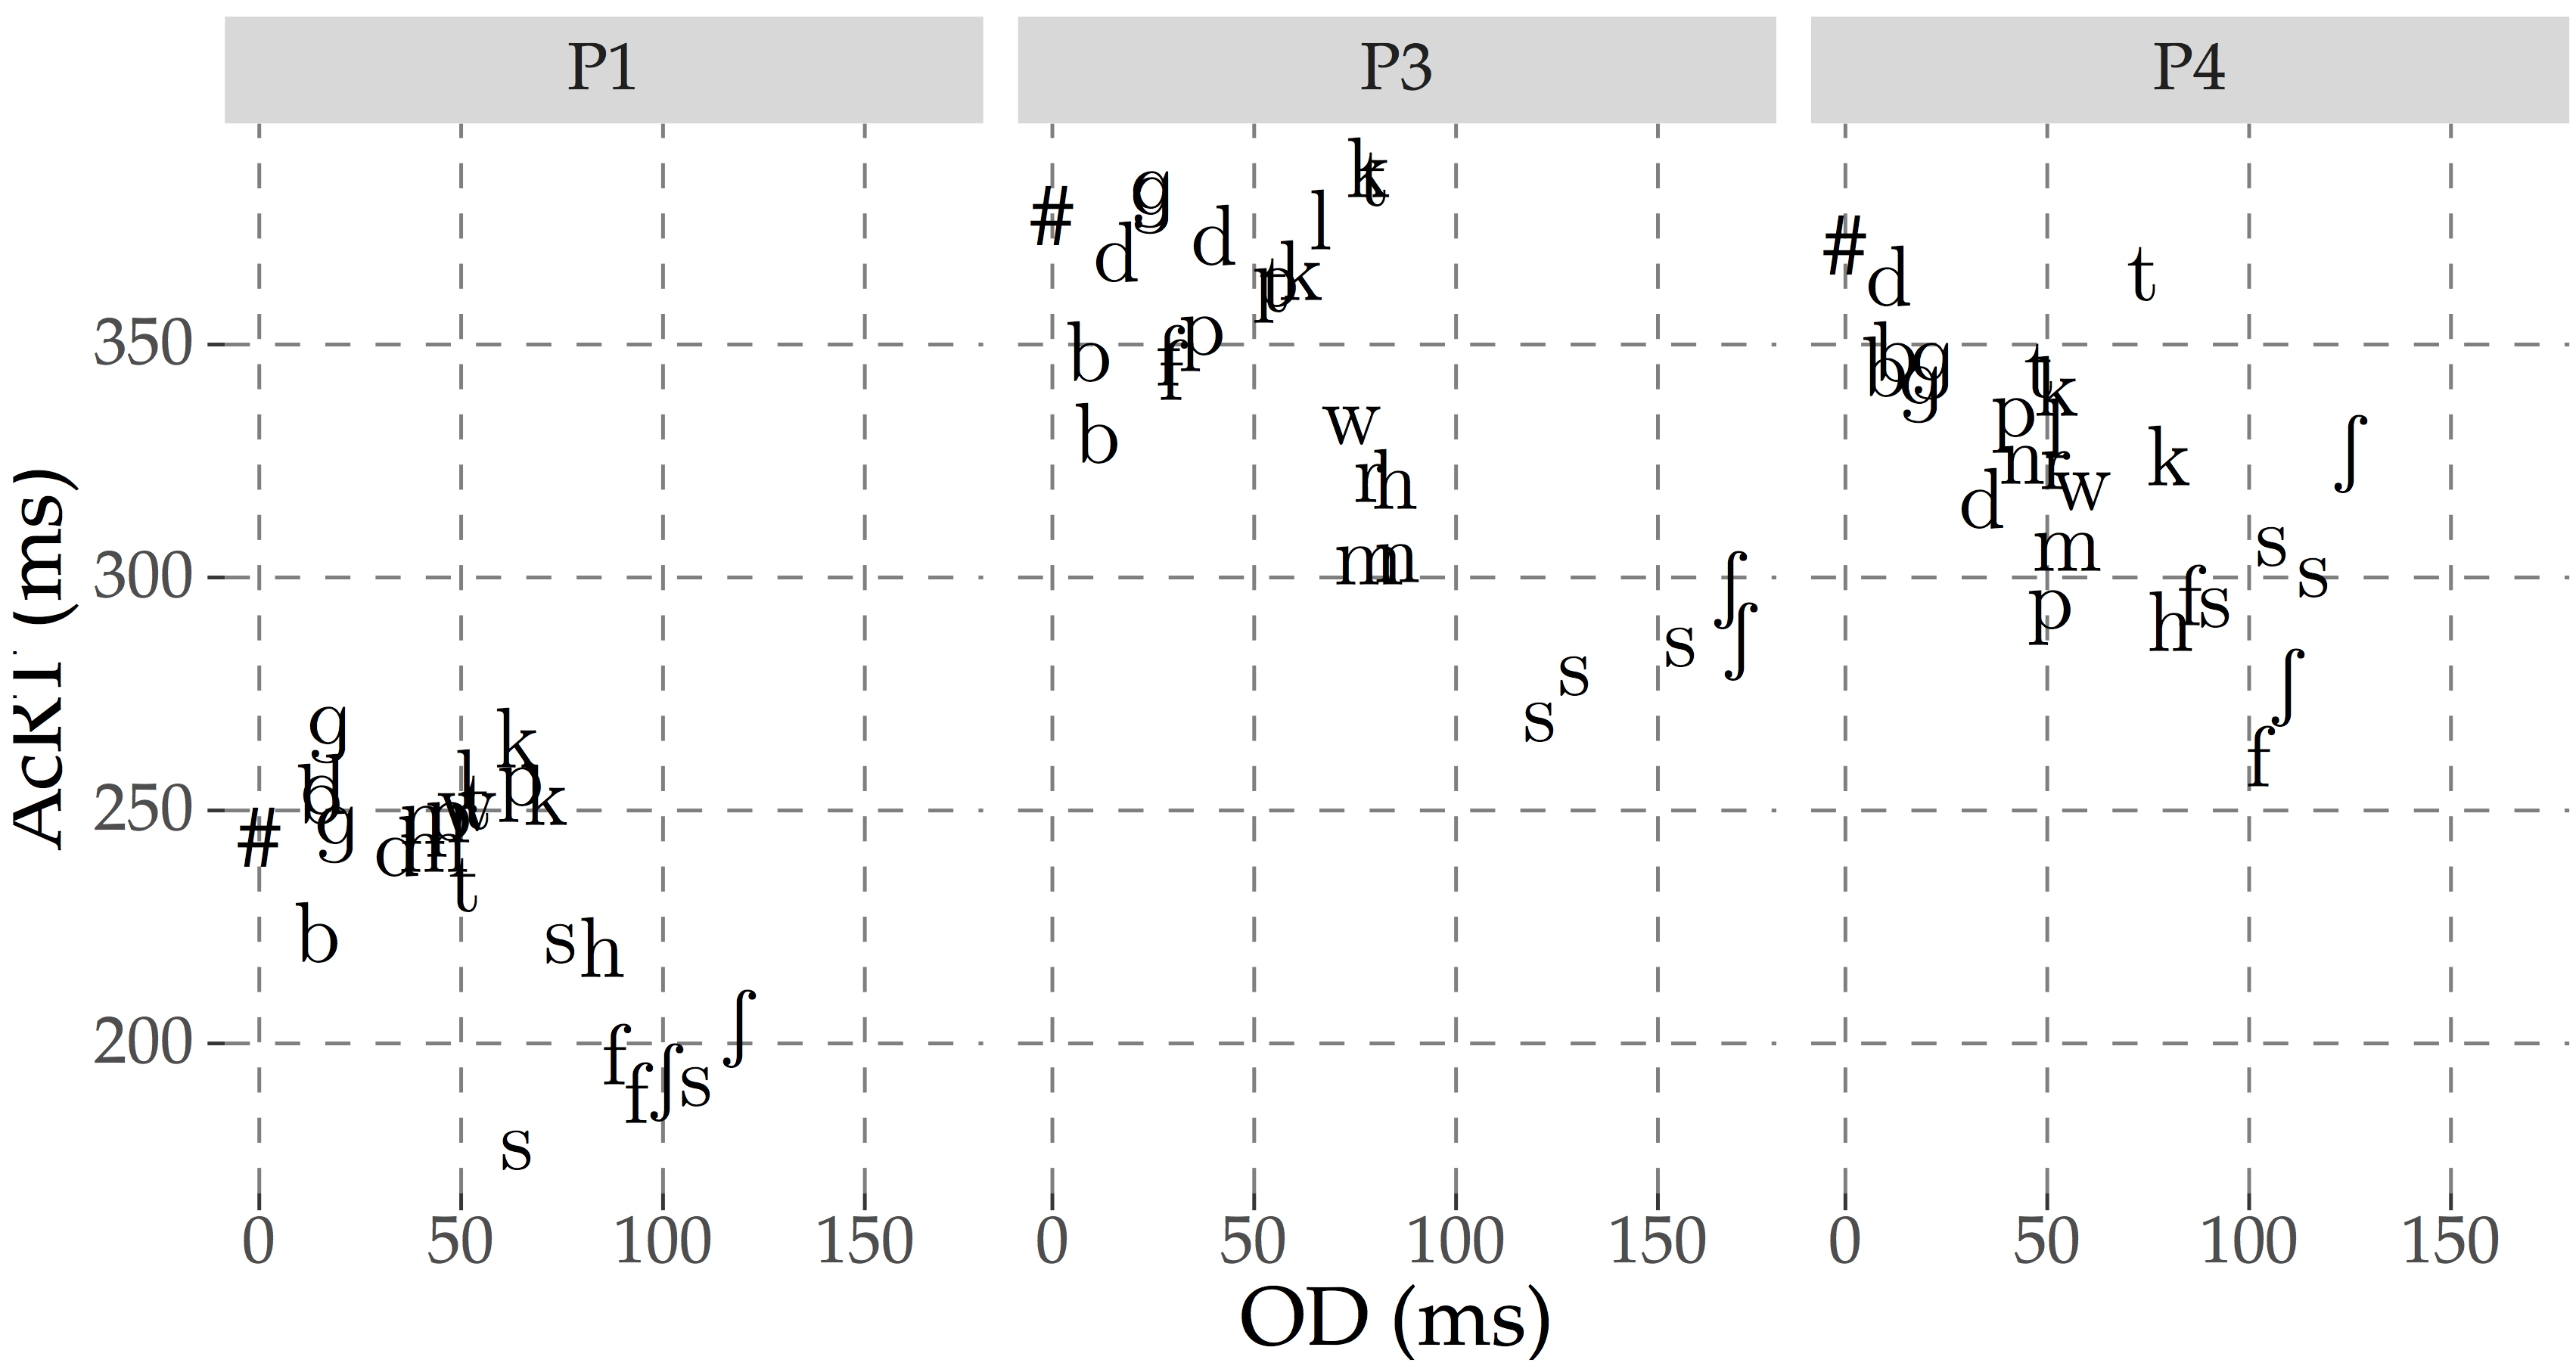
\includegraphics[width=\textwidth]{figures/OD_vs_AcRT.jpg}
	\end{center}
	Medianised within participant, over several repetitions and over
	the vowels \textipa{/a,i,O/}. Over all analysable n = 1386: 439 from P1, 672 from P3, and
	275 from P4.  }

\frame{\frametitle{Delayed naming results: Articulatory to Acoustic Interval}
	\begin{center}
		\vspace*{-.5cm}
		\hspace*{-1cm}
		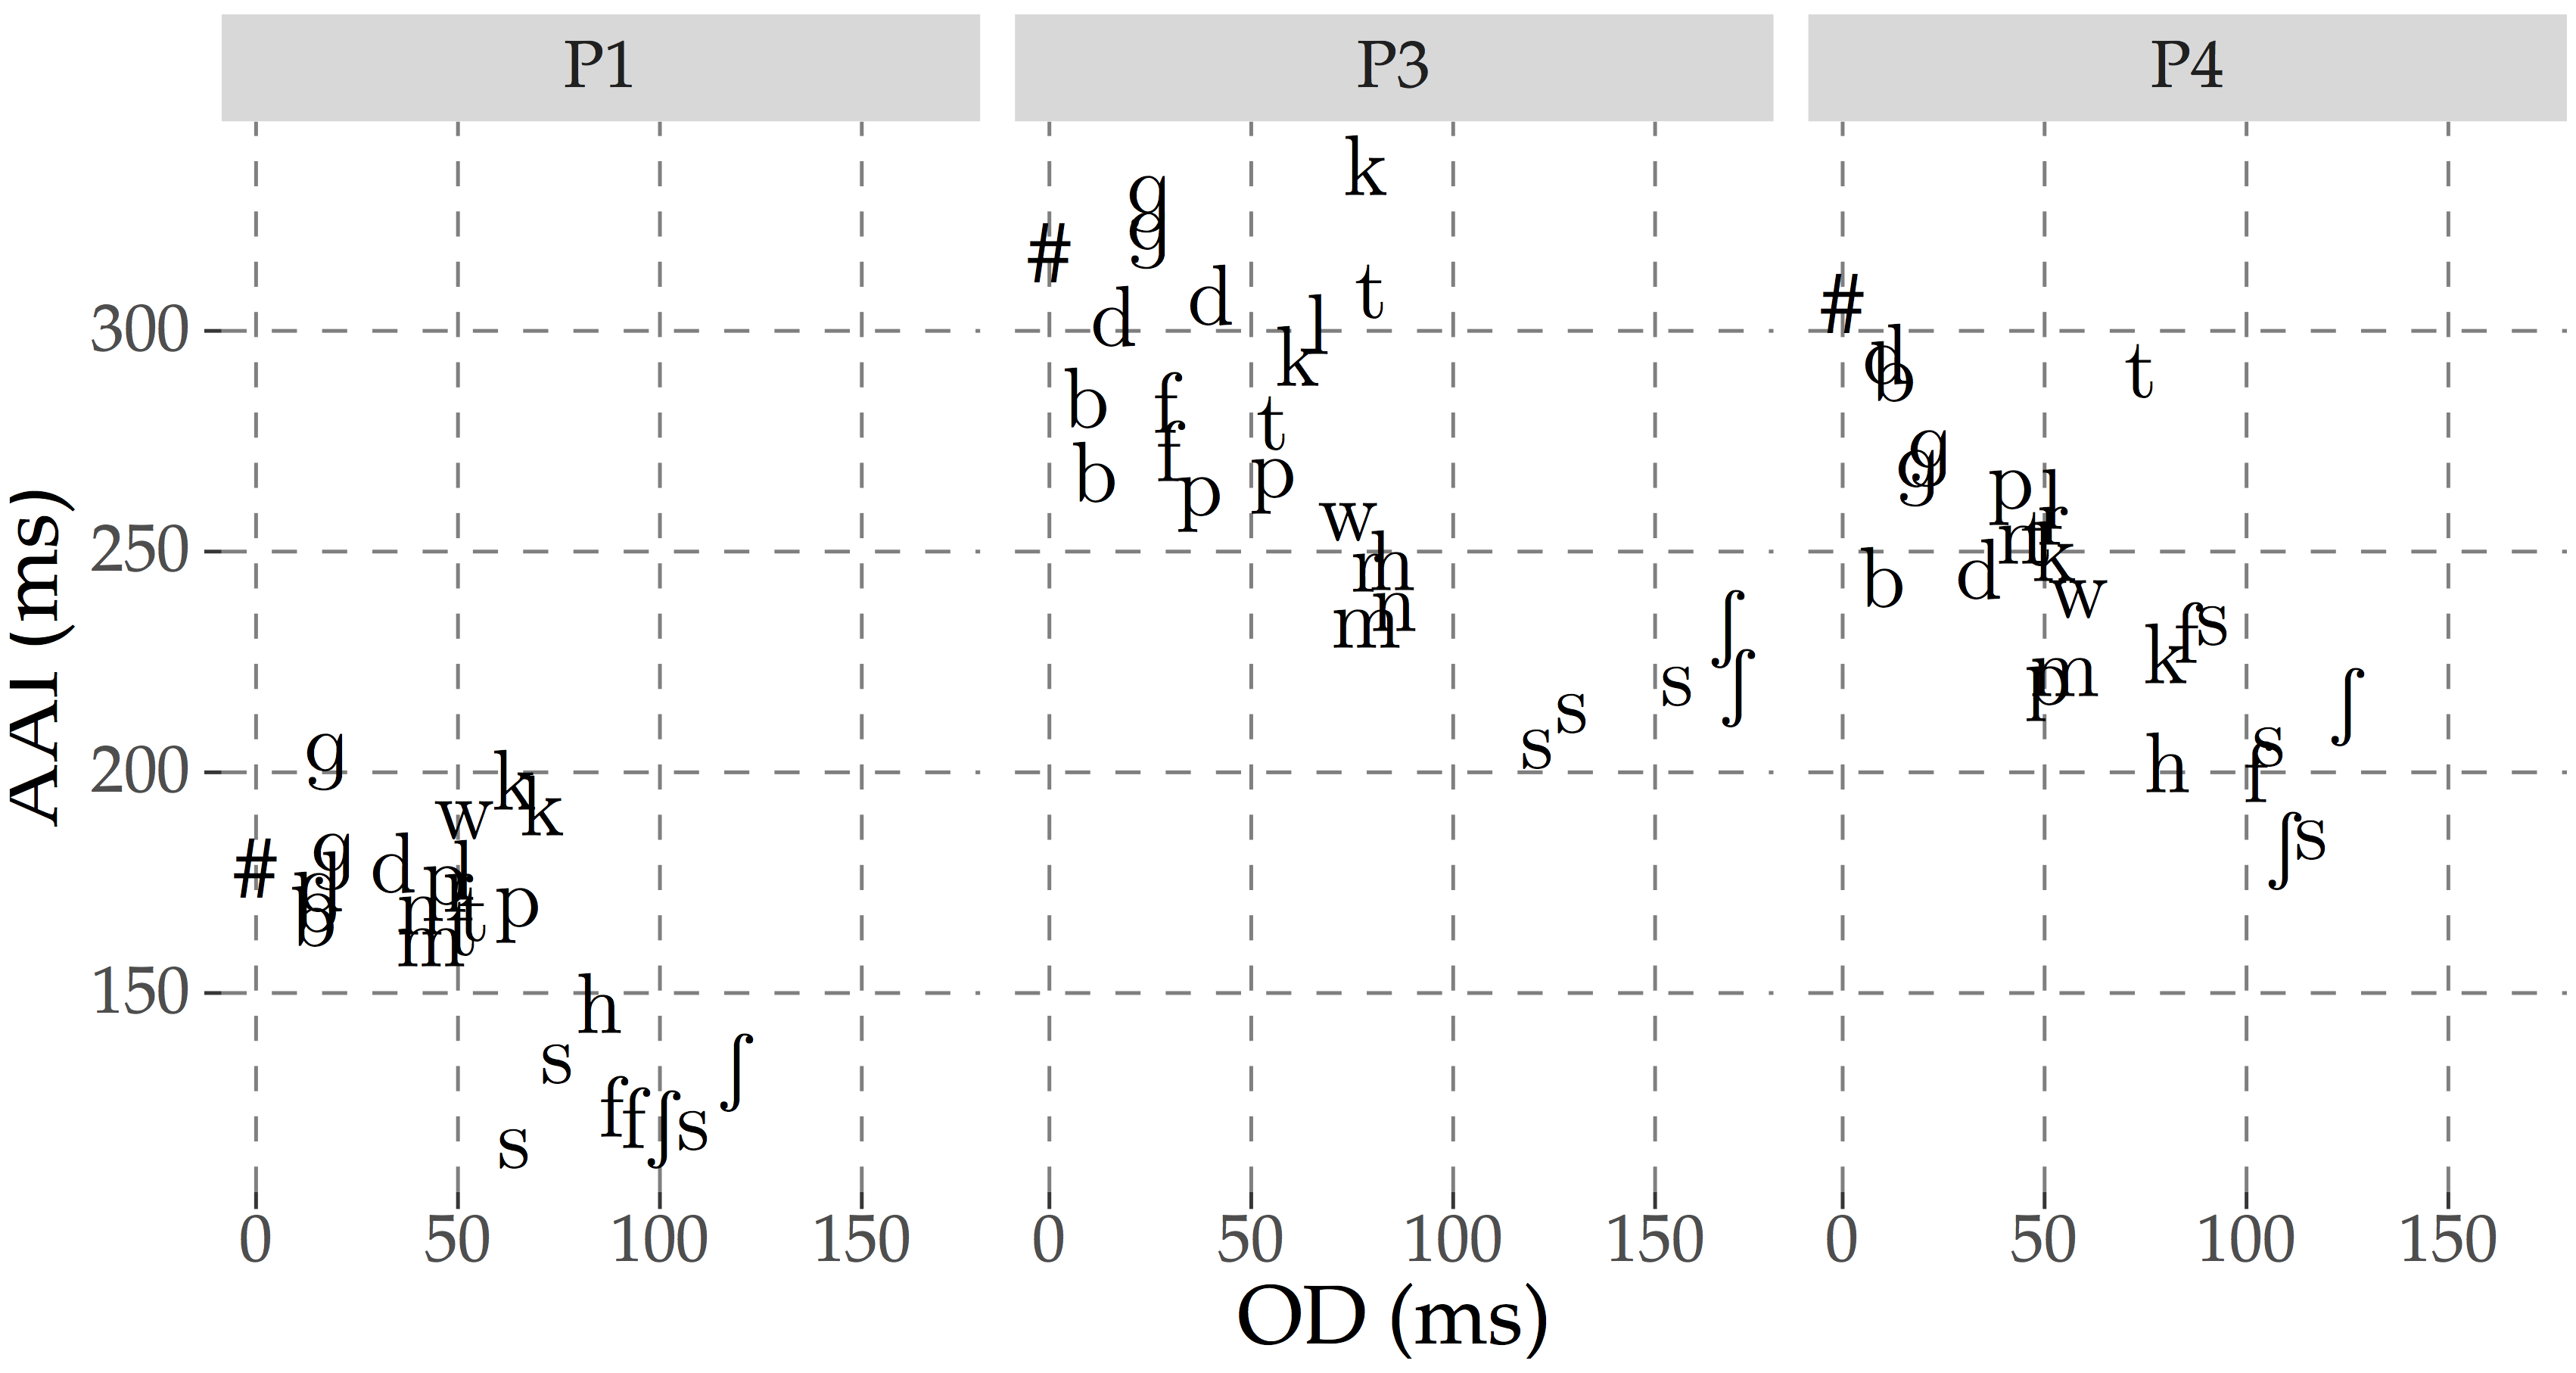
\includegraphics[width=\textwidth]{figures/OD_vs_AAI.jpg}
	\end{center}
	Medianised within participant, over several repetitions and over
	the vowels \textipa{/a,i,O/}. Over all analysable n = 1386: 439 from P1, 672 from P3,
	and 275 from P4.
}

\frame{\frametitle{Theory: Effect of OD on AAI}
	\begin{itemize}
		\item As the Onset Duration (OD) gets longer, Articulatory to Acoustic Interval (AAI) shortens.
		\item First three lines represent individual utterances, final line is a conceptual model of the effect of continuously lengthening OD.6
	\end{itemize}
	\begin{center}
		\hspace*{-.5cm}
		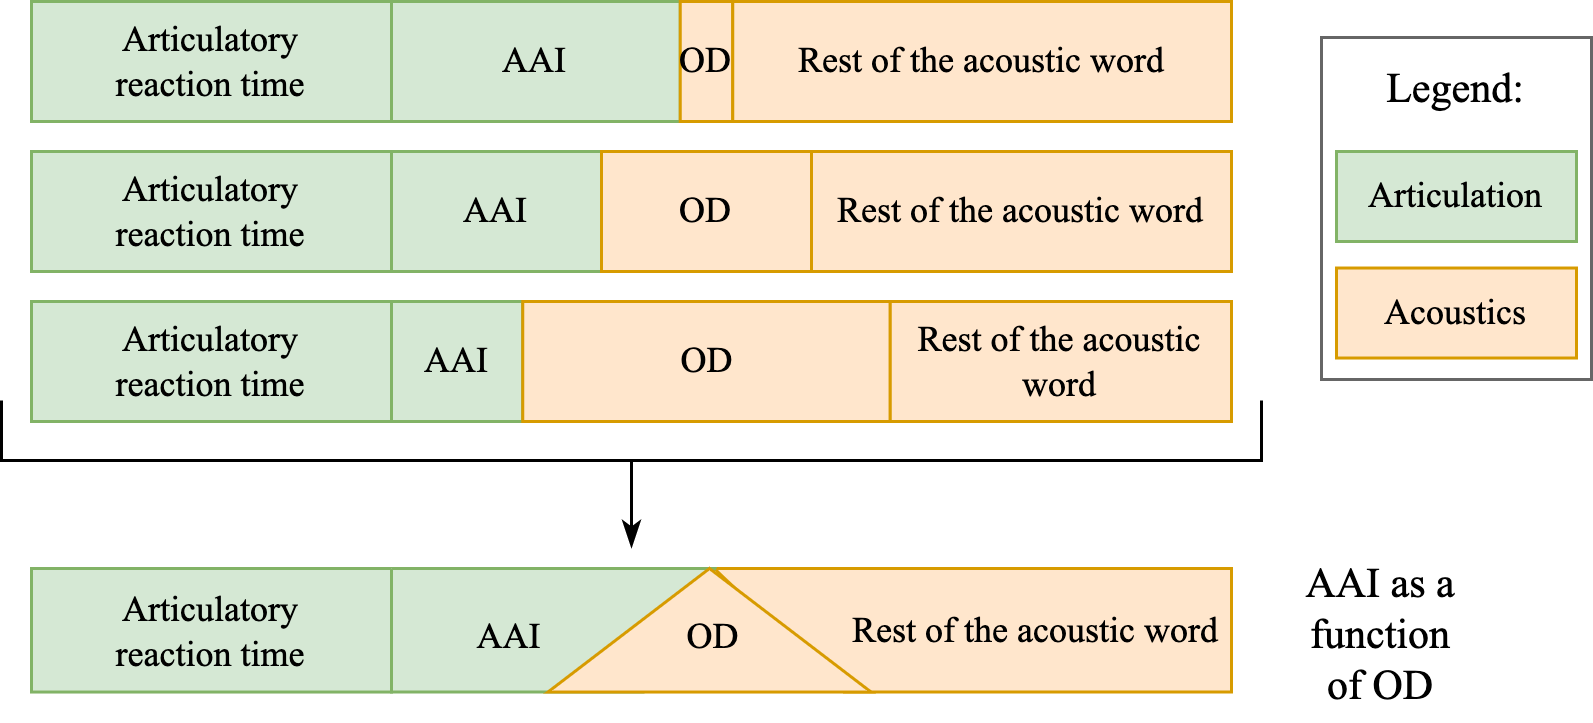
\includegraphics[width=1.1\textwidth]{effect_of_OD.drawio.png}
	\end{center}
}

\frame{\frametitle{Theory: Effect of articulatory rate on AAI}
	\begin{itemize}
		\item If we keep the utterance content constant but vary articulation rate, all parts (AAI, OD, and acoustic word) get longer as articulation rate goes down.
	\end{itemize}
	\begin{center}
		\hspace*{-.5cm}
		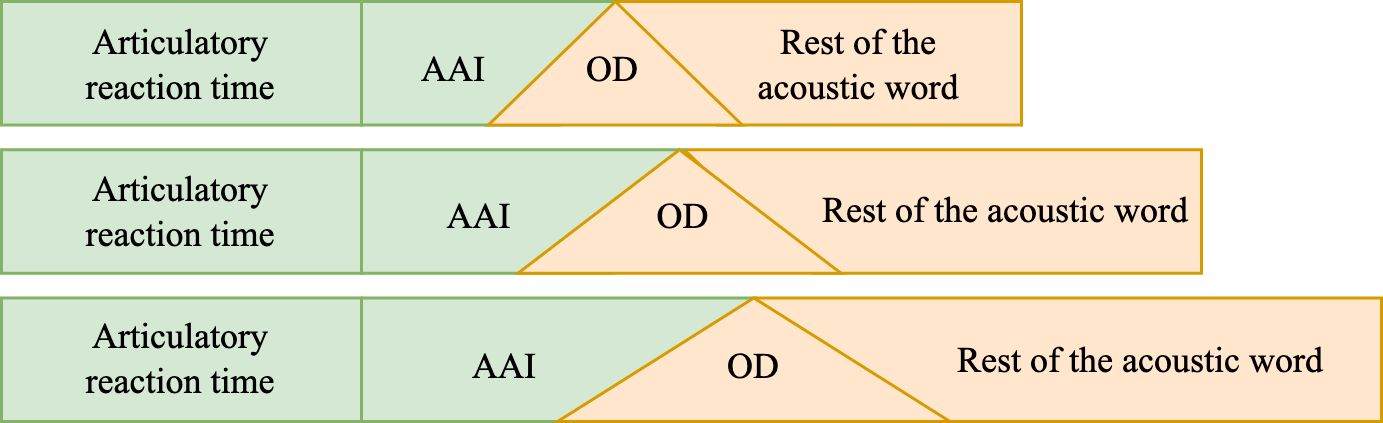
\includegraphics[width=\textwidth]{effect_of_RhymeDur.drawio.png}
	\end{center}
}

\end{document}

